% ==================================================================
% Compilation instructions:
% ------------------------------------------------------------------
% Use pdflatex to compile! Input images are expected as PDF files.
% Example compilation: 
% ------------------------------------------------------------------
% > pdflatex thesis-example.tex 
% > bibtex thesis-example
% > pdflatex thesis-example.tex 
% > pdflatex thesis-example.tex 
% ------------------------------------------------------------------
% You need to run pdflatex multiple times so that all the cross-references
% are fixed. pdflatex will tell you if you need to re-run it (a warning
% will be issued)
% ------------------------------------------------------------------
% Compilation has been tested to work in ukk.cs.hut.fi and kosh.hut.fi
% - if you have problems of missing .sty -files, then the local LaTeX
% environment does not have all the required packages installed.
% For example, when compiling in vipunen.hut.fi, you get an error that
% tikz.sty is missing - in this case you must either compile somewhere
% else, or you cannot use TikZ graphics in your thesis and must therefore
% remove or comment out the tikz package and all the tikz definitions.
% ------------------------------------------------------------------

% General information 
% ==================================================================
% Package documentation:
%
% The comments often refer to package documentation. (Almost) all LaTeX
% packages have documentation accompanying them, so you can read the
% package documentation for further information. When a package 'xxx' is
% installed to your local LaTeX environment (the document compiles
% when you have \usepackage{xxx} and LaTeX does not complain), you can
% find the documentation somewhere in the local LaTeX texmf directory
% hierarchy. In ukk.cs.hut.fi, this is /usr/texlive/2008/texmf-dist,
% and the documentation for the titlesec package (for example) can be
% found at /usr/texlive/2008/texmf-dist/doc/latex/titlesec/titlesec.pdf.
% Most often the documentation is located as a PDF file in
% /usr/texlive/2008/texmf-dist/doc/latex/xxx, where xxx is the package name;
% however, documentation for TikZ is in
% /usr/texlive/2008/texmf-dist/doc/latex/generic/pgf/pgfmanual.pdf
% (this is because TikZ is a front-end for PGF, which is meant to be a
% generic portable graphics format for LaTeX).
% You can try to look for the package manual using the ``find'' shell 
% command in Linux machines; the find databases are up-to-date at least
% in ukk.cs.hut.fi. Just type ``find xxx'', where xxx is the package
% name, and you should find a documentation file.
% Note that in some packages, the documentation is in the DVI file
% format. In this case, you can copy the DVI file to your home directory,
% and convert it to PDF with the dvipdfm command (or you can read the
% DVI file directly with a DVI viewer).
%
% If you can't find the documentation for a package, just try Googling
% for ``latex packagename''; most often you can get a direct link to the
% package manual in PDF format.
% ------------------------------------------------------------------

% Document class for the thesis is report
% ------------------------------------------------------------------
% You can change this but do so at your own risk - it may break other things.
% Note that the option pdftext is used for pdflatex; there is no
% pdflatex option.
% ------------------------------------------------------------------
\documentclass[12pt,a4paper,oneside,pdftex]{report} 

% The input files (tex files) are encoded with the latin-1 encoding
% (ISO-8859-1 works). Change the latin1-option if you use UTF8
% (at some point LaTeX did not work with UTF8, but I'm not sure
% what the current situation is)
\usepackage[utf8]{inputenc} 
% OT1 font encoding seems to work better than T1. Check the rendered
% PDF file to see if the fonts are encoded properly as vectors (instead
% of rendered bitmaps). You can do this by zooming very close to any letter
% - if the letter is shown pixelated, you should change this setting
% (try commenting out the entire line, for example).
\usepackage[OT1]{fontenc}
% The babel package provides hyphenating instructions for LaTeX. Give
% the languages you wish to use in your thesis as options to the babel
% package (as shown below). You can remove any language you are not
% going to use.
% Examples of valid language codes: english (or USenglish), british,
% finnish, swedish; and so on.
\usepackage[finnish,swedish,english]{babel}
\usepackage[sf]{titlesec}

\usepackage{float}

% Font selection
% ------------------------------------------------------------------
% The default LaTeX font is a very good font for rendering your
% thesis. It is a very professional font, which will always be
% accepted.
% If you, however, wish to spicen up your thesis, you can try out
% these font variants by uncommenting one of the following lines
% (or by finding another font package). The fonts shown here are
% all fonts that you could use in your thesis (not too silly).
% Changing the font causes the layouts to shift a bit; you many
% need to manually adjust some layouts. Check the warning messages
% LaTeX gives you.
% ------------------------------------------------------------------
% To find another font, check out the font catalogue from
% http://www.tug.dk/FontCatalogue/mathfonts.html
% This link points to the list of fonts that support maths, but
% that's a fairly important point for master's theses.
% ------------------------------------------------------------------

%\usepackage{tgcursor}
%\usepackage{nimbus}
%\usepackage[scaled]{helvet}
%\renewcommand*\familydefault{\sfdefault} %% Only if the base font of the document is to be sans serif
% \usepackage{palatino}
% \usepackage{tgpagella}

\usepackage[scaled]{helvet}
%\usepackage{sectsty}
%\allsectionsfont{\ttfamily}
%\usepackage{courier}
\usepackage[bitstream-charter]{mathdesign}

% Optional packages
% ------------------------------------------------------------------
% Select those packages that you need for your thesis. You may delete
% or comment the rest.

% Natbib allows you to select the format of the bibliography references.
% The first example uses numbered citations:
% \usepackage[square,sort&compress,numbers]{natbib}
% The second example uses author-year citations.
% If you use author-year citations, change the bibliography style (below);
% acm style does not work with author-year citations.
% Also, you should use \citet (cite in text) when you wish to refer
% to the author directly (\citet{blaablaa} said blaa blaa), and
% \citep when you wish to refer similarly than with numbered citations
% (It has been said that blaa blaa~\citep{blaablaa}).
\usepackage[round]{natbib}

% The alltt package provides an all-teletype environment that acts
% like verbatim but you can use LaTeX commands in it. Uncomment if
% you want to use this environment.
% \usepackage{alltt}

% The eurosym package provides a euro symbol. Use with \euro{}
\usepackage{eurosym}

% Verbatim provides a standard teletype environment that renderes
% the text exactly as written in the tex file. Useful for code
% snippets (although you can also use the listings package to get
% automatic code formatting).
\usepackage{verbatim}

% The listing package provides automatic code formatting utilities
% so that you can copy-paste code examples and have them rendered
% nicely. See the package documentation for details.
% \usepackage{listings}

% The fancuvrb package provides fancier verbatim environments
% (you can, for example, put borders around the verbatim text area
% and so on). See package for details.
% \usepackage{fancyvrb}

% Supertabular provides a tabular environment that can span multiple
% pages.
%\usepackage{supertabular}
% Longtable provides a tabular environment that can span multiple
% pages. This is used in the example acronyms file.
\usepackage{longtable}
\usepackage[table]{xcolor}

% The fancyhdr package allows you to set your the page headers
% manually, and allows you to add separator lines and so on.
% Check the package documentation.
% \usepackage{fancyhdr}

% Subfigure package allows you to use subfigures (i.e. many subfigures
% within one figure environment). These can have different labels and
% they are numbered automatically. Check the package documentation.
\usepackage{subfigure}

% The titlesec package can be used to alter the look of the titles
% of sections, chapters, and so on. This example uses the ``medium''
% package option which sets the titles to a medium size, making them
% a bit smaller than what is the default. You can fine-tune the
% title fonts and sizes by using the package options. See the package
% documentation.
\usepackage[medium]{titlesec}

% The TikZ package allows you to create professional technical figures.
% The learning curve is quite steep, but it is definitely worth it if
% you wish to have really good-looking technical figures.
\usepackage{tikz}
% You also need to specify which TikZ libraries you use
\usepackage{censor}

\usepackage{enumitem}
\usepackage{changepage}
\usetikzlibrary{positioning}
\usetikzlibrary{calc}
\usetikzlibrary{arrows}
\usetikzlibrary{decorations.pathmorphing,decorations.markings}
\usetikzlibrary{shapes}
\usetikzlibrary{patterns}
\usetikzlibrary{chains}
\usetikzlibrary{backgrounds, fit}

% The aalto-thesis package provides typesetting instructions for the
% standard master's thesis parts (abstracts, front page, and so on)
% Load this package second-to-last, just before the hyperref package.
% Options that you can use:
%   mydraft - renders the thesis in draft mode.
%             Do not use for the final version.
%   doublenumbering - [optional] number the first pages of the thesis
%                     with roman numerals (i, ii, iii, ...); and start
%                     arabic numbering (1, 2, 3, ...) only on the
%                     first page of the first chapter
%   twoinstructors  - changes the title of instructors to plural form
%   twosupervisors  - changes the title of supervisors to plural form
\usepackage[twosupervisors]{aalto-thesis}
%\usepackage[mydraft,doublenumbering]{aalto-thesis}
%\usepackage{aalto-thesis}

% Hyperref
% ------------------------------------------------------------------
% Hyperref creates links from URLs, for references, and creates a
% TOC in the PDF file.
% This package must be the last one you include, because it has
% compatibility issues with many other packages and it fixes
% those issues when it is loaded.
\RequirePackage[pdftex]{hyperref}
% Setup hyperref so that links are clickable but do not look
% different
\hypersetup{colorlinks=false,raiselinks=false,breaklinks=true}
\hypersetup{pdfborder={0 0 0}}
\hypersetup{bookmarksnumbered=true}
% The following line suggests the PDF reader that it should show the
% first level of bookmarks opened in the hierarchical bookmark view.
\hypersetup{bookmarksopen=true,bookmarksopenlevel=1}
% Hyperref can also set up the PDF metadata fields. These are
% set a bit later on, after the thesis setup.

% Thesis setup
% ==================================================================
% Change these to fit your own thesis.
% \COMMAND always refers to the English version;
% \FCOMMAND refers to the Finnish version; and
% \SCOMMAND refers to the Swedish version.
% You may comment/remove those language variants that you do not use
% (but then you must not include the abstracts for that language)
% ------------------------------------------------------------------
% If you do not find the command for a text that is shown in the cover page or
% in the abstract texts, check the aalto-thesis.sty file and locate the text
% from there.


% All the texts are configured in language-specific blocks (lots of commands
% that look like this: \renewcommand{\ATCITY}{Espoo}.
% You can just fix the texts there. Just remember to check all the language
% variants you use (they are all there in the same place).
% ------------------------------------------------------------------
\newcommand{\TITLE}{IT CAN FELL ROCKETS}
\newcommand{\FTITLE}{Automaatiokehys integraatioiden regressiotestaukseen}
\newcommand{\SUBTITLE}{or developing a framework for continuous integration testing at a lifecycle power solutions supplier}
\newcommand{\FSUBTITLE}{}
\newcommand{\DATE}{August 12, 2013}
\newcommand{\FDATE}{12. elokuuta 2013} % Todo, poista draft
\newcommand{\SDATE}{Den 12 augusti 2013}

% Supervisors and instructors
% ------------------------------------------------------------------
% If you have two supervisors, write both names here, separate them with a
% double-backslash (see below for an example)
% Also remember to add the package option ``twosupervisors'' or
% ``twoinstructors'' to the aalto-thesis package so that the titles are in
% plural.
% Example of one supervisor:
%\newcommand{\SUPERVISOR}{Professor Antti Ylä-Jääski}
%\newcommand{\FSUPERVISOR}{Professori Antti Ylä-Jääski}
%\newcommand{\SSUPERVISOR}{Professor Antti Ylä-Jääski}
% Example of twosupervisors:
\newcommand{\SUPERVISOR}{Professor Riitta Smeds}
\newcommand{\FSUPERVISOR}{Professori Riitta Smeds}
\newcommand{\SSUPERVISOR}{Professor Riitta Smeds}

% If you have only one instructor, just write one name here
\newcommand{\INSTRUCTOR}{Eero Tuomikoski M.Sc. (Tech.)\\ Inka Vilpola D.Sc. (Tech.)}
\newcommand{\FINSTRUCTOR}{Diplomi-insinööri Eero Tuomikoski\\ Tekniikan tohtori Inka Vilpola}
\newcommand{\SINSTRUCTOR}{Diplomingenjör Eero Tuomikoski\\ Doktor Inka Vilpola}

% If you have two instructors, separate them with \\ to create linefeeds
% \newcommand{\INSTRUCTOR}{Olli Ohjaaja M.Sc. (Tech.)\\
%  Elli Opas M.Sc. (Tech)}
%\newcommand{\FINSTRUCTOR}{Diplomi-insinööri Olli Ohjaaja\\
%  Diplomi-insinööri Elli Opas}
%\newcommand{\SINSTRUCTOR}{Diplomingenjör Olli Ohjaaja\\
%  Diplomingenjör Elli Opas}

% If you have two supervisors, it is common to write the schools
% of the supervisors in the cover page. If the following command is defined,
% then the supervisor names shown here are printed in the cover page. Otherwise,
% the supervisor names defined above are used.
\newcommand{\COVERSUPERVISOR}{Professor Riitta Smeds, Aalto University}

% The same option is for the instructors, if you have multiple instructors.
% \newcommand{\COVERINSTRUCTOR}{Olli Ohjaaja M.Sc. (Tech.), Aalto University\\
%  Elli Opas M.Sc. (Tech), Aalto SCI}

% Other stuff todo
% ------------------------------------------------------------------
\newcommand{\PROFESSORSHIP}{ Business and Service Processes in Digital Networks}
\newcommand{\FPROFESSORSHIP}{Liiketoimintaverkostot}
\newcommand{\SPROFESSORSHIP}{}
% Professorship code is the same in all languages
\newcommand{\PROFCODE}{TU-124}
\newcommand{\KEYWORDS}{integration testing, testing automation, testing framework, continuous integration, software testing}
\newcommand{\FKEYWORDS}{regressiotestaus, ohjelmistotestaus, automatisoitu testaus, integraatiotestaus, testikehys, jatkuva testaus}
\newcommand{\SKEYWORDS}{testning}
\newcommand{\LANGUAGE}{English}
\newcommand{\FLANGUAGE}{englanti}
\newcommand{\SLANGUAGE}{Engelska}

% Author is the same for all languages
\newcommand{\AUTHOR}{Antti Heikkonen}

% Currently the English versions are used for the PDF file metadata
% Set the PDF title
\hypersetup{pdftitle={\TITLE\ \SUBTITLE}}
% Set the PDF author
\hypersetup{pdfauthor={\AUTHOR}}
% Set the PDF keywords
\hypersetup{pdfkeywords={\KEYWORDS}}
% Set the PDF subject
\hypersetup{pdfsubject={Master's Thesis}}

% Layout settings
% ------------------------------------------------------------------

% When you write in English, you should use the standard LaTeX
% paragraph formatting: paragraphs are indented, and there is no
% space between paragraphs.
% When writing in Finnish, we often use no indentation in the
% beginning of the paragraph, and there is some space between the
% paragraphs.

% If you write your thesis Finnish, uncomment these lines; if
% you write in English, leave these lines commented!
% \setlength{\parindent}{0pt}
% \setlength{\parskip}{1ex}

% Use this to control how much space there is between each line of text.
% 1 is normal (no extra space), 1.3 is about one-half more space, and
% 1.6 is about double line spacing.
% \linespread{1} % This is the default
% \linespread{1.3}

% Bibliography style
% acm style gives you a basic reference style. It works only with numbered
% references.
% \bibliographystyle{acm}
% Plainnat is a plain style that works with both numbered and name citations.
\bibliographystyle{kbib}


% Extra hyphenation settings
% ------------------------------------------------------------------
% You can list here all the files that are not hyphenated correctly.
% You can provide many \hyphenation commands and/or separate each word
% with a space inside a single command. Put hyphens in the places where
% a word can be hyphenated.
% Note that (by default) LaTeX will not hyphenate words that already
% have a hyphen in them (for example, if you write ``structure-modification
% operation'', the word structure-modification will never be hyphenated).
% You need a special package to hyphenate those words.
\hyphenation{di-gi-taa-li-sta yksi-suun-tai-sta}

% The preamble ends here, and the document begins.
% Place all formatting commands and such before this line.
% ------------------------------------------------------------------
\begin{document}
% This command adds a PDF bookmark to the cover page. You may leave
% it out if you don't like it...
\pdfbookmark[0]{Cover page}{bookmark.0.cover}
% This command is defined in aalto-thesis.sty. It controls the page
% numbering based on whether the doublenumbering option is specified
\startcoverpage

% Cover page
% ------------------------------------------------------------------
% Options: finnish, english, and swedish
% These control in which language the cover-page information is shown
\coverpage{english}

% Abstracts
% ------------------------------------------------------------------
% Include an abstract in the language that the thesis is written in,
% and if your native language is Finnish or Swedish, one in that language.

% Abstract in English
% ------------------------------------------------------------------
\thesisabstract{english}{

Software integration is an assembly task where components have to be laid carefully for seamless interoperation. One ill-advised change in either the integrations, or inside the systems themselves, might potentially cause a harmful discontinuity in daily operations. This master's thesis examines testing these cross-component and cross-system connections within a Finnish complete lifecycle power solutions supplier and sets out to define a practical method of operation for conducting automated integration testing.

The thesis expounded on integration testing theory and frameworks. Testing frameworks in academic literature were deconstructed and analyzed, and their characteristic features observed. These practical insights were combined with theoretical findings and crystallized into a new integration testing framework, which was then tailored for case company needs. The resulting framework was comprehensively evaluated through requirements analysis, heuristic appraisal, and qualitative validation by company experts. 

The constructed framework both describes testing process work flow and suggests technical implementation. In practice, the implementation brings a sense of organization to a previously ad hoc process thereby mitigating business risk. In theory, it extends the popular notion that integration testing is a mere transitional period in development and examines testing as a continuous process all the way from the strategic level to the mundane. The thesis constitutes a cohesive narrative and guide to implementing automated integration testing.

}

% Abstract in Finnish
% ------------------------------------------------------------------
\thesisabstract{finnish}{
Ohjelmistot rakentuvat useiden komponenttien ja järjestelmien yhteistoiminnasta. Näiden \emph{integraatioiden} ja rajapintojen toimivuus ja toimintavarmuus on tärkeää. Yksinkin muutos jossakin integraatiossa tai osajärjestelmässä voi vaarantaa liiketoiminnan jatkuvuuden. Tämä diplomityö tutkii, mitä automatisoidulta integraatiotestaukselta edellytetään ja, perustuen kohdeyrityksen vaatimuksiin, minkälainen toimintatapa vastaa integraatiotestaustarvetta.

Tutkimus pureutui ohjelmistotestausmalleihin ja -teorioihin ja se suoritettiin suomalaisen konepajayhtiön tilauksesta. Se tarkasteli aikaisemman akateemisen tutkimuksen testikehyksiä ja perusteellisesti selvitti mistä osista nämä koostuvat. Näistä kehysten ja testausteorian havainnosta rakennettiin uusi testikehys, joka myös perustui kohdeyrityksen vaatimuksiin. Kehyshypoteesia arvioitiin huolellisesti testauksen vaatimusten, ohjelmistokehyksien heuristiikkojen ja asiantuntijalausuntojen avulla.

Työn tuloksena on suositus testikehyksen työnkululle ja prosesseille, sekä kehyksen käytännön toteutukselle. Uusi kehys kääntää testauksen satunnaisesta hallituksi ja järjestelmälliseksi prosessiksi parantaen samalla liiketoimintariskien hallintaa. Kehyksen tausta-ajatuksena on myös haastaa yleinen käsitys siitä, että integraatiotestaus on pelkkä ohjelmistokehityksen välivaihe. Se tarkasteleekin testausta jatkuvana prosessina aina strategiselta tasolta päivittäiseen ja komponenttitasoon. Tutkimuksen kaari muodostaa ehyen kertomuksen ja käsikirjan automatisoidun integraationtestauksen toteuttamisesta.

}

% Acknowledgements
% ------------------------------------------------------------------
% Select the language you use in your acknowledgements
\selectlanguage{english}

% Uncomment this line if you wish acknoledgements to appear in the
% table of contents
%\addcontentsline{toc}{chapter}{Acknowledgements}

% The star means that the chapter isn't numbered and does not
% show up in the TOC
\chapter*{Acknowledgements}

Making this thesis has been a fun and wholly rewarding exploration of the murky waters around organizational regression testing. Throughout the researching and writing I was helped by many who deserve my sincere gratitude. I wish to thank Wärtsilä's technical experts for their advice and enthusiasm in the project, my friends and peers for their useful suggestions and feedback, my thesis supervisor for her open-minded, but grounded encouragement, and finally, and in particular, my instructors for their enduring support.

Thank you, and remember --- test often, and test early.
\vskip 10mm

\noindent Helsinki, \DATE
\vskip 5mm
\noindent\AUTHOR

% Acronyms
% ------------------------------------------------------------------
% Use \cleardoublepage so that IF two-sided printing is used
% (which is not often for masters theses), then the pages will still
% start correctly on the right-hand side.
\cleardoublepage
% Example acronyms are placed in a separate file, acronyms.tex
% \input{acronyms}

\addcontentsline{toc}{chapter}{Abbreviations and Acronyms}
\chapter*{Abbreviations and Acronyms}

% The longtable environment should break the table properly to multiple pages,
% if needed

\noindent

\begin{longtable}{@{}p{0.25\textwidth}p{0.7\textwidth}@{}}

ANT & A Java library and command-line capable of driving sofware engineering processes, such as compiling, assembling, and testing, described in build files as targets and extension points dependent upon each other. \citep{ant2013} \\[0.3cm]

Black-box testing & A testing strategy that considers a functional design specification to design test cases without regard to internal program structure. \citep{burnstein2003practical} \\[0.3cm]

CI & See \emph{continuous integration}. \\[0.3cm]

Capture and playback & See \emph{record and playback} \\[0.8cm]

Bug & See \emph{defect}. \\[0.3cm]

Component testing & Testing a collection of units which together form a single component or module, or testing component-based systems in general. \citep{wu2003uml, ieee2010systems} \\[0.3cm]

Continuous integration & A development practice where team members integrate their work frequently and each integration is verified by an automated build which include tests to detect flaws as quickly as possible. \citep{fowler2006continuous} \\[0.3cm]

Defect & A flaw in the system or component that causes it to fail to perform its function. \citep{burnstein2003practical, ieee2010systems} \\[0.3cm]

ESB & \textbf{E}nterprise \textbf{S}ervice \textbf{B}us. \emph{"An Enterprise Service Bus is an open standards, messagebased, distributed integration infrastructure that provides routing, invocation and mediation services to facilitate the interactions of disparate distributed applications and services in a secure and reliable manner."} \citep{menge2007enterprise, tuomikoski2010monitoring} \\[0.3cm]

Failure & The state or event of failing to meet specified expectations or objectives. \citep{ieee2010systems} \\[0.3cm]

Fault & A defect in the software which may lead to a \emph{failure}. \citep{ieee2010systems} \\[0.3cm] 

Fault-based testing & Using information about previous failures to design system specifications and test cases. Also: purposely inserting faults into the system and then measuring the effectiveness of the test suite in finding them. \citep{pezze2008software} \\[0.3cm]  

Framework & An abstract design which can be extended by adding more or better components to it. Unlike libraries, the framework often plays the role of the main program in coordinating and sequencing application activity. \citep{laukkanen2006data, ieee2010systems}  \\[0.3cm]

Functional testing & \emph{Black-box testing} conducted to evaluate the compliance of a system or component with specified functional requirements. \citep{ieee2010systems} \\[0.3cm] 

IEEE & \textbf{I}nstitute of \textbf{E}lectrical and \textbf{E}lectronics \textbf{E}ngineers. Professional association for the advancement of technology. IEEE issues publications, organizes conferences, compiles standards, and organizes various professional and educational activities. \citep{ieee2013} \\[0.3cm] 

Integration testing & An orderly progression of testing where individual software and hardware elements are combined and tested until entire the system has been integrated. \citep{burnstein2003practical} Testing in which \emph{"software components, hardware components, or both are combined and tested to evaluate the interaction among them"} \citep{ieee2010systems} A level of test undertaken to validate the interface between internal components of a system. Typically based upon the system architecture. \citep{craig2002systematic} \\[0.3cm]

Library & \emph{"A controlled collection of software and related documentation designed to aid in software development, use, or maintenance."} See also \emph{framework}. \citep{ieee2010systems} \\[0.3cm]

Model-based testing & A testing approach where test cases are automatically derived from architectural and behavioural models and specifications. \citep{apfelbaum1997model} \\[0.3cm]

Mock service & A simulated software component simulating a one function or service. May have been constructed through \emph{record and replay} or a \emph{surrogate engine}. \\[0.3cm]

Non-functional testing & Testing non-functional qualities of software, e.g. usability, performance, conformity, security, etc. Non-functional requirements specify not what the software will do but how the software will do it. \citep{ieee2010systems} \\[0.3cm]

Record and playback & An approach where a test tool records test input and outcomes and provides facilities for subsequent re-execution or replay of the test. \citep{burnstein2003practical, ieee2010systems} \\[0.3cm]

Regression testing & Selective re-execution of tests on software that has been modified to ensure that no defects have been introduced by the modification and that the software still satisfies its specification. \citep{burnstein2003practical, ieee2010systems} \\[0.3cm]

Retesting & The re-execution of tests in order to verify that a defect has been correctly fixed. \citep{jenkins2008software} \\[0.3cm]

SOA & \textbf{S}ervice-\textbf{O}riented \textbf{A}rchitecture. A software architecture design pattern based on structured collections of discrete software modules, or services, which together provide the full functionality of a large software application. \citep{velte2009cloud} \\[0.3cm]

Surrogate or surrogate engine & A simulation apparatus that is capable of creating and running surrogate components which simulate unavailable system services or components. See also \emph{mock service}. \\[0.3cm]

Stub & A simulation of a particular sub-component which can be used to simulate that component in a larger assembly. \citep{jenkins2008software} Program logic substituting for the body of a software component that is or will be defined elsewhere. \citep{ieee2010systems} \\[0.3cm]

System testing & \emph{"The process of testing an integrated hardware and software system to verify that the system meets its specified requirements."} \citep{burnstein2003practical} \\[0.3cm]

SUT & \textbf{S}ystem \textbf{U}nder \textbf{T}est. The entire system or product that is tested. \citep{craig2002systematic} \\[0.3cm]

Test case & A test-related item which contains test inputs, execution conditions, and expected outputs. \citep{burnstein2003practical, ieee2010systems} \\[0.3cm]

Test framework & A \emph{framework} used for testing. \\[0.3cm]

Test harness & A configuration of surrogate components which substituting for parts of the deployment environment. \citep{pezze2008software} \\[0.3cm]

Test oracle & A piece of software which applies pass and fail criterion to a program execution. \citep{pezze2008software}. \\[0.3cm] 

Test set &  A collection of one or more test cases. \\[0.3cm] %

Test suite & See \emph{test set}. \\[0.3cm] 

Unit testing & The \emph{"aggregate of technical activities involved in demonstrating that an individual software unit has been implemented correctly, and that the code and the design of a unit are consistent, and that the unit design is correct."} \citep{burnstein2003practical} \\[0.3cm]

Validation & The process of evaluating a software system or component during or at the end of the development phase to evaluate whether it meets the customer requirements. \citep{ieee2010systems} \\[0.3cm]

Verification & \emph{"The process of evaluating a software system or component to determine whether the products of a given development phase satisfy the conditions composed at the start that phase."} \citep{ieee2010systems} \\[0.3cm]

White-box testing & A testing strategy that requires knowledge of the internal structure of a program to design test cases \citep{burnstein2003practical} \\[0.3cm]

WSDL & \textbf{W}eb \textbf{S}ervice \textbf{D}escription \textbf{L}anguage. An XML-based language defining web service interfaces. \citep{christensen2001web} \\[0.3cm]

XML & \textbf{E}xtensible \textbf{M}arkup \textbf{L}anguage.  A markup language to describe and define other human and machine-readable formats and encodings. \citep{w32013}\\[0.3cm]

\end{longtable}

% Table of contents
% ------------------------------------------------------------------
\cleardoublepage
% This command adds a PDF bookmark that links to the contents.
% You can use \addcontentsline{} as well, but that also adds contents
% entry to the table of contents, which is kind of redundant.
% The text ``Contents'' is shown in the PDF bookmark.
\pdfbookmark[0]{Contents}{bookmark.0.contents}
\tableofcontents

% List of tables
% ------------------------------------------------------------------
% You only need a list of tables for your thesis if you have very
% many tables. If you do, uncomment the following two lines.
% \cleardoublepage
% \listoftables

% Table of figures
% ------------------------------------------------------------------
% You only need a list of figures for your thesis if you have very
% many figures. If you do, uncomment the following two lines.
% \cleardoublepage
% \listoffigures

% The following label is used for counting the prelude pages
\label{pages-prelude}
\cleardoublepage

%%%%%%%%%%%%%%%%% The main content starts here %%%%%%%%%%%%%%%%%%%%%
% ------------------------------------------------------------------
% This command is defined in aalto-thesis.sty. It controls the page
% numbering based on whether the doublenumbering option is specified
\startfirstchapter

% Add headings to pages (the chapter title is shown)
\pagestyle{headings}

% The contents of the thesis are separated to their own files.
% Edit the content in these files, rename them as necessary.
% ------------------------------------------------------------------

% \input{1introduction.tex}
\chapter{Introduction}
\label{chapter:introduction}
% Keywords: system-to-system integration (testing), automated testing, testing framework, integration testing

% there exists process for general test design, prioritizing, planning, identifying test data, the framework focuses on test execution and making testing technically possible, testing policy, communication, environment, test suite and maintenance, practical process for test execution, reporting

% Something to grab the reader's attention
\begin{adjustwidth}{2.5em}{0pt}
\small
\textbf{\emph{On June 4th 1996, just 37 seconds after its launch off the Guiana Space Centre in French Guiana, carrier rocket Ariane 5 self-destructs in a magnificent spectral burst after veering off course, its navigation software toppled by a measly integer overflow. One the most costly software bugs in history, the Ariane rocket failure losses have been estimated at over 300 million euros. \citep{dowson1997ariane}}}
\normal
\end{adjustwidth}
\vspace{8 mm}

At the confluence of cognition lies danger --- but also great potential. Integrating disparate tasks to achieve one complex end result greater than the sum of its parts embodies the same principles as the division of labour. Complex problems are easier to solve when divided, each part administered by a dedicated expert; cooperation fosters growth. 

Integrating information systems is common practice in organizations and corporations, too, and often a prerequisite for operational IT in the modern networked business landscape. Information, the very same information, must be available and at the disposal of multiple interconnected systems worldwide. At the same time, researchers like \citet{myers1976software} and \citet{reid2005art} have estimated that testing and maintenance costs amount to over 50\% of total software costs, compelling to organize testing cost-effectively.

The sporadically distributed systems do have many advantages. They bear the brunt of clerical work and and handle transactional communication with mathematical precision. They enable incremental growth, either through conscious extension of services or a less conscious natural evolution and accretion of new services. Other benefits of an interdependent and connected information technology system include a reduction in the number of systems related upkeep, maintenance, and development costs. Shared resources bring economies of scale as software components find reuse. \citep{rehman2007testing} Having fewer systems also reduces the degree of complexity in the organisational IT set-up.

\begin{comment}
% benefits of automation, build-up to integration, orienting to automated IT business processes
%start with key concept, not automation, real-time processes perspective, inter-company, information flow as a % reason, add picture and figure, why was the work conducted? business critical and dependencies. why?
Automation is one of the great boons brought on by technological development on one hand freeing up resources like labour for more value-adding purposes --- and permitting the execution of uniform, repeatable processes and process control on the other. The pinnacle of advancement and prosperity on which society stands today is based on a continuous flow of various automated tasks and electronic services, many of which are complex and involve a slew of actors or agents. Work is divided and its completion therefore requires cooperation between service systems.
\end{comment}

However, integration efforts may result in unclear responsibilities and difficulties in determining if the systems cooperate and behave correctly, and if any use cases are unaccounted for. In a distributed system there are more component dependencies and connections that can fail. Relinquishing control over units always carries risk that they'll be ill-managed by someone who has misunderstood priorities or ambitions. Typically integrations are tested after the developer passes the unit-tested software on to the tester or end user and not always do the two sides see eye to eye. A high number of interdependent integrations makes the task even more daunting since a single change in the system components can disrupt a whole chain of operations and the integration house of cards comes tumbling down as was the case with the Ariane 5 rocket \citep{pezze2008software, rehman2007testing}.

% business motivation and technical considerations
The benefits outweighing all shortcomings, modern corporations' business processes rely on automated IT and operate on distributed systems and networked devices. But the problems are still there. Therefore, ensuring quality of service is essential. Systematic, rigorous, and preferably automated regression testing, both functional and non-functional, is needed to maintain a requisite degree of confidence in the performance and serviceability of information systems. \citet{rehman2007testing} call it an \emph{"indispensible testing phase"}. This thesis examines the requirements of system-to-system integration testing both in a theoretical and a real world business setting, constructs a testing paradigm to mediate over integration issues, and tries it out in practice. The supposition is that a carefully crafted framework will help uncover defects and issues earlier and more efficiently, and help resolve them with fewer resources.

This thesis studies system integration testing at a Finnish complete lifecycle power solutions supplier Wärtsilä. Wärtsilä's IT systems are mediated over a central hub, the enterprise service bus. Messages travelling between two systems go through integration modules and procedures built around the bus. Since critical systems are connected via the hub it has itself become very critical for business continuity. Moreover, since new services and systems are constantly being introduced and old ones updated, there exists a continuing need for retesting the system integrations. Even if the applications change only a little, there exists a significant risk that something has broken \citep{pezze2008software}. 
%Define it for savings and communicate to external stakeholders.

% since executed by a push of a button, human dimension not needed. however: application responsibilities and installation and configuration, creating new test cases, framework requires support. normally process chart has actors on y column, here difficult to plot. mapping tasks to people left out of scope (test planner, test) 

\section{Research questions}

The overall purpose of the study is to devise a testing framework for automated integration tests. Here, \emph{'framework'} refers to both the structure and configuration of the technical testing solution, as well as the process structure. This is then subjected to qualitative evaluation in a workshop at the case company after which a revised version of it is presented. A prototype is created in the vein of constructive research to help evaluate the framework applicability.

Testing involves many managerial aspects, tasks, and responsibilities navigating the maze of stakeholders and scheduling manual work. This thesis only examines the technical process requirements of automated integration testing and the manual work needed to maintain it. It is a manual on the process of how to build a framework and will only expand on the framework's implementation from a technical point of view. Defect or incident management, as well as implementing the change, are left out of the thesis scope.
% is the ways of working

The research problem can be divided into two questions: \\

% 1. Determine requirements.
\begin{adjustwidth}{2.5em}{0pt}
\textbf{1. What are the requirements for an automated integration testing framework?} \\
\end{adjustwidth}

The first research question addresses the pertinent subquestions: what is a framework and how should integration testing be conducted? Based on academic literature, the integration testing framework is modelled and its constituent processes are described, which also serves as a foundation for answering the second research question.

The first part then proceeds to requirements analysis and uncovering the criteria for a suitable framework structure. These requirements are based on Wärtsilä's operational IT environment as well as generic observations made earlier in the study. Wärtsilä's system environment and electronic business processes and integrations are a canonical example of corporate IT and as such should lend themselves well to comparison to previous research. \\

% , consisting for instance between the ERP system and warehouse systems, and the ERP system and the PDM system which should lend itself well to comparisons to previous research.\\

\begin{adjustwidth}{2.5em}{0pt}
\textbf{2. How should the testing framework be constructed and maintained?} \\
\end{adjustwidth}

The latter research question beckons to a practical constructive approach. To determine the right processes and tools for the framework a proof of concept construct is made and, in the terms of the industry, \emph{smoke tested} for any immediate faults. The actual implementation or adoption of the presented test framework is \textbf{not} part of the thesis.

Answering the second research question also includes evaluation of how the end solution meets previously defined criteria and requirements. Any other issues and concerns that arise during the experiment part are also discussed.

An additional outcome, a set of implementation guidelines and recommendations that is based on observed results and conclusions, was produced and attached to the study (see Appendix \ref{chapter:guidelines-appendix}).

The framework technology evaluation and choice is omitted from the scope of the thesis, though reasons for the ultimate framework tool choice are given and derived from Wärtsilä's requirements. Fit for the purpose of the assignment, quick assessment is used to determine a set of alternatives that are easy to use and satisfy the framework requirements. Going through a screened set of available tools and analyzing and quantifying their potential steps across to decision-making science and is therefore out of the thesis scope. 

% b meyer: ironic that more computing power does not yield better tests, process contains bottlenecks of manual tasks

\section{Research method}
% not to produce hard fact to the academic canon
Research follows the constructive research method --- a six step model, where a concrete, real world problem is investigated through practical experience and academic understanding \citep{kasanen1993constructive}. The resulting conclusions and concepts are then tested in a working simulation. The emphasis is to produce hypotheses and theories, and test them in practice reflecting and appraising the theoretical groundwork laid earlier in research. The constructive research elements are depicted in Figure \ref{fig:constructive} while the steps include \citep{kasanen1993constructive}:
\\
\begin{adjustwidth}{2.5em}{0pt}
\small
\begin{enumerate}[itemsep=0mm]
\item Find a practically relevant problem which also has research potential.
\item Obtain a general and comprehensive understanding of the topic.
\item Innovate, i.e., construct a solution idea.
\item Demonstrate that the solution works.
\item Show the theoretical connections and the research contribution of the solution concept.
\item Examine the scope of applicability of the solution.
\end{enumerate}
\normal
\end{adjustwidth}

\vspace{6 mm}

As a scientific work, and to satisfy the first two steps, the thesis's research problem must be relevant enough to be interesting, and robust enough for academic research. The third crucial step entails the construction of a novel solution and new understanding, which are then argued in step four, with the purpose of demonstrating that the built construct works. In the fifth step the researcher compares the solution to theoretical models and in the final step evaluates its applicability in light of the original research problem, thesis scope, and in the idealized theoretical setting. Constructive research highlights the pragmatic applicability of the solution including aspects of quality, cost, and timeliness.

\begin{figure}[H]
\centering
% =================================================
\pgfdeclarelayer{marx}
\pgfsetlayers{main,marx}
% -------------------------------------------------
% Start the picture
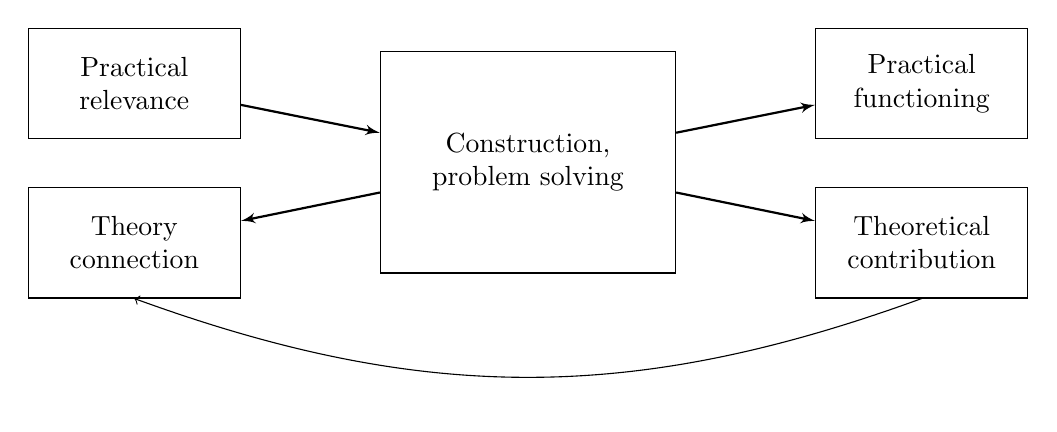
\begin{tikzpicture}[
    start chain=going below,    % General flow is top-to-bottom
    node distance=6mm and 50mm, % Global setup of box spacing
    ]
% ------------------------------------------------- 
\tikzset{
  base/.style={draw, on chain, on grid, align=center, minimum height=4ex},
  proc/.style={base, rectangle, minimum height=4em, text width=7em},
  big/.style={base, rectangle, minimum height=8em, text width=10em},
   line/.style={draw, thick, -latex'}
}
% -------------------------------------------------
% Placing the nodes

\node [proc] (rel) {Practical relevance};
\node [proc] (con) {Theory connection};
\node [big, right=of rel, yshift=-1cm] (prb) {Construction, problem solving};
\node [proc, right=of prb, yshift=1cm] (fun) {Practical functioning};
\node [proc] (ctr) {Theoretical contribution};

\path [line] (rel) -- (prb);
\path [line] (prb) -- (fun);
\path [line] (prb) -- (ctr);
\path [line] (prb) -- (con);
%\path [line] (ctr) -- (con);
\draw[->] (ctr.south) to [out=-160,in=-20] (con.south);

\end{tikzpicture}
\caption{Constructive research model adapted from \citet{kasanen1993constructive}} \label{fig:constructive}
\end{figure}

Reasoning follows an abductive logic path where an initial observation in the "real" world is brought under theoretical scrutiny and modelling. The phenomenon is then subjected to experiments to shape a general conclusion. \citep{josephson1996abductive} The subsequent rationalisation is the then returned to inductive empirical appraisal and generalized back into theory and a new, refined model. 

\section{Thesis structure}
\label{section:structure} 

This master's thesis study is divided into eight parts. First, necessary background information on software integration testing, case company Wärtsilä's systems architecture, and information systems is presented in Chapter \ref{chapter:background}. The chapter also includes a requirements analysis based on interviews conducted at the company. Next, integration testing frameworks are explored by looking at existing models and a synthesis on their strategic, tactical, and operational nature is given. Along with a more generic look at integration testing theory, Chapter \ref{chapter:frameworkanalysis} breaks down the framework into process components, which are then put together in Chapter \ref{chapter:frameworkproposal} into a new framework model tailored for Wärtsilä.

% testing automation are examined. efficient defect management. 
The empirical part of the study evaluates a working prototype of the new testing framework. It presents a proof-of-concept implementation and reflects on the solution in respect to previous academic research and applicability in solving Wärtsilä's underlying business problems. The last chapters contains critical appraisal of both the theoretical and empirical part of the study and if the thesis met its objectives while also discussed implications and limitations of study. 

The rough frame of study is pictured in Figure \ref{fig:thesisstructure}.

\begin{figure}[H]
\centering
% =================================================
\pgfdeclarelayer{marx}
\pgfsetlayers{main,marx}
% -------------------------------------------------
% Start the picture
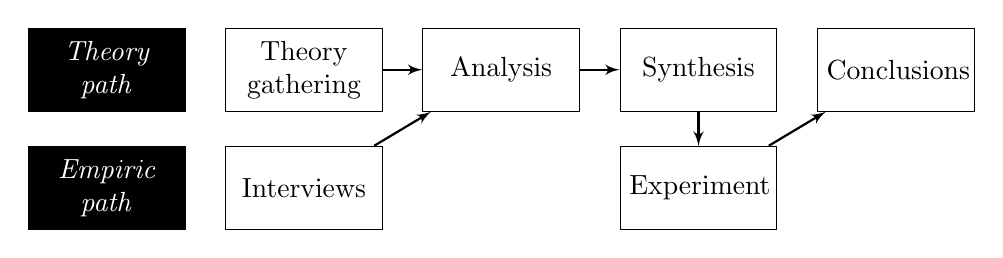
\begin{tikzpicture}[
    start chain=going right,    % General flow is top-to-bottom
    node distance=15mm and 5mm, % Global setup of box spacing
    ]
% ------------------------------------------------- 
\tikzset{
  base/.style={draw, on chain, on grid, align=center, minimum height=3ex},
  proc/.style={base, rectangle, minimum height=3em, text width=5em},
  blank/.style={base, fill=black, text=white, rectangle, minimum height=3em, text width=5em},
   line/.style={draw, thick, -latex'}
}
% -------------------------------------------------
% Placing the nodes

\node [blank] (tpt) {\emph{Theory path}};
\node [proc] (thr) {Theory gathering};
\node [proc] (anl) {Analysis};
\node [proc] (syn) {Synthesis};
\node [proc] (con) {Conclusions};

\node [blank, below=of tpt] (ept) {\emph{Empiric path}};
\node [proc, below=of thr] (int) {Interviews};
\node [proc, below=of syn] (exp) {Experiment};

\path [line] (int) -- (anl);
\path [line] (thr) -- (anl);
\path [line] (anl) -- (syn);
\path [line] (syn) -- (exp);
\path [line] (exp) -- (con);

\end{tikzpicture}
\caption{Thesis structure} \label{fig:thesisstructure}
\end{figure}

In a manner of speaking, the story arc of the thesis is like putting together Lego. In the background chapter (Chapter \ref{chapter:background}) the constructor can peruse the contextual setting and rough guidelines for assembly, while in the next part, he/she is shown ready models, built by experts, for reference and inspiration. After this, the box is merrily torn open and the bricks scattered on the floor. The builder can pore over individual pieces and see how they they appear, feel, and stick together. A prototype construct is made and compared to expectations and presented to experts and interested parties. Finally a new, better version of the construct is documented and discussed.

\chapter{Research background}
\label{chapter:background}

% defining process, financal gain tied to company objectives
% what should be measured? add to workshop agenda?
% rquirements analysis should be done well so as to avoind further issues or issues in commuication
% process must be defined first, then the actual IT system
% 1. haasteet 2. käyttäjät 3. käyttötapaukset 4. tietosisältöjen määrittely

To help fully grasp the key questions in the thesis, the reader is furnished with necessary background information about software (integration) testing, its merits, and the testing need at Wärtsilä. The theoretical and practical insights serve as reference when constructing the testing framework.

The first two chapters examine software testing from a more general perspective. The method of research is literature study. The latter two chapters investigate Wärtsilä's context of need and enumerates requirements for the framework, which are based on interviews with testing and solution experts at Wärtsilä.

\section{Testing software systems}

Testing is an essential part of software engineering. Without a degree of confidence of sound operation and functional integrity, systems accumulate great risk and may ultimately produce more harm than benefit. Controlled testing reduces the number of incidents that would otherwise be discovered in the live environment and fixing which would be very expensive. \citep{jenkins2008software, liu2009unified} In a similar fashion, testing can point to ways the systems can be improved. For example, a system that is fluid and easy to use does not incur as many service and maintenance or information requests. And lastly, testing helps decision makers understand the risks involved in IT applications and services.

Along with the functionality of the system, tests should also be applied to non-functional aspects such as performance and usability, because these also determine the validity of the system under test (SUT). Verifying that specified functions are implemented is not enough, but the system must reach and perform at an adequate level of service. In practice, performance testing is impossible without some form of computer-controlled execution of tests \citep{laukkanen2006data}.

Traditionally, testing is grouped to \emph{unit}, \emph{integration}, and \emph{system} levels \citep{jenkins2008software, burnstein2003practical}. Unit testing is assuring that individual software modules and functions perform to specifications. When these are paired or grouped, the resulting connections and integrations must also be tested. Typically this is done by the solution users as opposed to developers who usually perform unit testing. Finally, system testing refers to proofing the finished software suite with a suitable array of use cases. It also includes load and performance tests. \citep{rehman2007testing}

The distinction between unit, integration, and system tests is not clear, however. Some authors \citep{tsai2001end, paul2001end} consider end-to-end integration testing akin to system tests. \citet{duvall2007continuous} writes about \emph{component testing} synonymous with integration testing. \citet{pezze2008software} and \citet{benz2007combining} consider this an intermediary stage between unit and integration/system tests while \citet{burnstein2003practical} likens component testing to unit testing. \citet{ieee2010systems} defines integration testing as testing in which \emph{"software components, hardware components, or both are combined and tested to evaluate the interaction among them"}.

% What to test
The fluid progression from atomic unit tests to holistic system tests strongly reflects the software development process. Naturally, software has to be tested to during and after initial development, but there are other reasons, too. Any change in code or specifications, the environment, or testing policy, or plans can act as a trigger for testing. Systematically repeating a set of tests to ascertain changes (like fixes) have not introduced new errors to previously functional code is called regression testing. The execution of regression tests is particularly suited for automation and executing all applicable tests just in case a common strategy \citep{jenkins2008software, pezze2008software}. A nearby concept, \textit{retesting} refers to examining if a fix has actually resolved a software bug \citep{jenkins2008software}.

Continuous integration (CI) is a further approach where testing is done frequently as changes are made to source code. The purpose is to weed out issues and defects related to component inter-operation before they take root can cause major trouble. \citet{fowler2006continuous} described continuous integration as:

\begin{adjustwidth}{2.5em}{0pt}
\small
\emph{"A software development practice where members of a team integrate their work frequently, usually each person integrates at least daily --- leading to multiple integrations per day. Each integration is verified by an automated build (including test) to detect integration errors as quickly as possible. Many teams find that this approach leads to significantly reduced integration problems and allows a team to develop cohesive software more rapidly."}
\normal
\end{adjustwidth}

% move integration testing stuff here?
% maturity increase - > support integatration cost and time decrease 90 %

\section{Why automated testing?}

% Write about what processes are already defined and argue that there is no overlap. What to do. technique how to do. Does not assume overall test steering responsibilities, the two are separated and not dependent so they can be updated individually.

The bigger and the more numerous information systems are, the more problems are likely to arise. Software failures may result in squandered time and money, and even loss of life \citep{leveson1993investigation, defense1992software}. The growing pressures for delivering quality and controlling IT risks are reflected on software testing. This in turn creates a demand for testing automation. Already in 1976 \citet{myers1976software} stated that maintenance and testing account for 75\% of software costs.

The oft-cited reasons for testing automation are improving software quality and cost-efficiency: harnessing the power of computers helps expedite the testing process as well as reduce the amount of manual work. \citet{fewster1999software} give a more complete list of automation benefits:

\begin{itemize}
\item Reusing tests on a new version of the system
\item Reusing tests in a new project
\item Running tests more often
\item Performing tests which would be difficult or impossible to do manually (e.g. performance tests)
\item Freeing test engineers to do more rewarding work
\item Consistency and repeatability of tests
\item Increased confidence due to increased and systematic testing
\item Shortening development time, faster time to market
\end{itemize}

Naturally, automation comes with its downsides and risks, some of which are not insignificant. These will be explored later in Section \ref{section:pitfalls}.

\section{Testing at Wärtsilä}

% tähänkö esittely?
Wärtsilä is a Finnish technology company providing lifecycle power solutions for the marine and energy markets. Of the three main business units Ship Power provides complete offerings of marine products and integration solutions for various segments like the Offshore and Cruise Ship markets, Power Plants designs and constructs plants, and Services offer a range of maintenance services and support to Wärtsilä's customers. \citep{wartsila2013web}

% add mention of interview

Integration testing is particularly important at Wärtsilä because the company typically outsources IT development. This pushes unit testing responsibilities to the supplier, while solution integration remains Wärtsilä's concern and responsibility. A flexible and well-defined integration testing process framework can serve many development projects to come. To date, there have been cases with unnecessary duplicate work. In a recent ERP update effort the scale of and need for testing became evident to Wärtsilä. A framework guiding the testing process and automating a part of it could significantly reduce costs and risks as well as project execution time.

% references to these? what can be included?
Wärtsilä's business rests on over a thousand systems of which about 50 are integrated over the service bus. These include for example enterprise and customer resource planning, product data management, warehouse control, and financial systems, which are intersected by information exchange processes. Applications are managed by experts known as Solution Managers who maintain the services and provide support for users.

The system architecture is built on the service-orientation principle (SOA), where individual systems or software components lend their services to be called by other systems' services through a shared channel, the enterprise service bus (ESB) \citep{tuomikoski2010monitoring}. Adapters and application programming interfaces (APIs) provide a means to access and use systems irrespective of their internal composition (e.g. programming language). This permits adding new services and replacing or removing old ones incrementally, but does not remove the challenges related to testing. A change in even one of the systems can potentially break one or more process chains.

% remove picture?
\begin{figure}
\centering
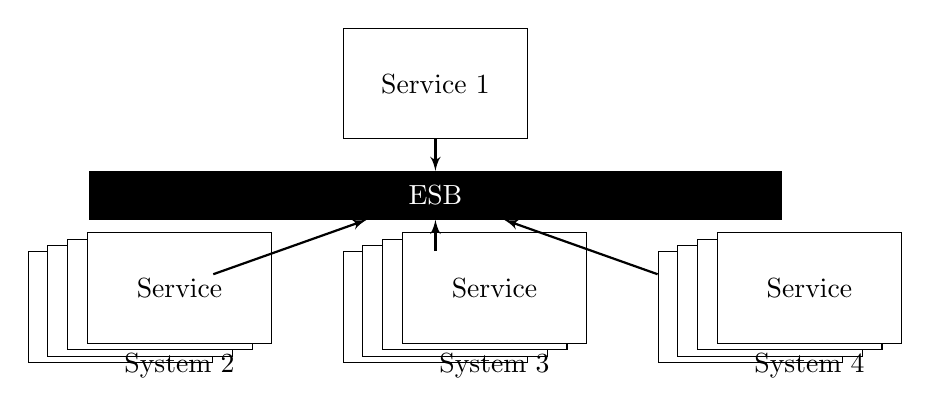
\begin{tikzpicture} [
   start chain=going below,        % General flow is top-to-bottom
    node distance=4mm and 40mm,    % Global setup of box spacing
    ]
% ------------------------------------------------- 
\tikzset{
  base/.style={draw, on chain, on grid, align=center, minimum height=4ex},
  rect/.style={base, rectangle, minimum height=4em, text width=6em},
  bus/.style={base, rectangle, minimum width=25em, fill=black, text=white, text width=8em},
  line/.style={draw, thick, -latex'},
}
    \node [rect, xshift=1.25cm] (s1) {Service 1};
    \node [bus] (esb) {ESB};
  
    \node [rect, xshift=-4.00cm] (s21) {};
    \node [rect, xshift=0.25cm, yshift=1.90cm, fill=white] (s22) {};
    \node [rect, xshift=0.25cm, yshift=1.90cm, fill=white] (s23) {};
    \node [rect, xshift=0.25cm, yshift=1.90cm, fill=white, label=below:{System 2}] (s24) {Service};
    
    \node [rect, right=of s21] (s31) {};
    \node [rect, xshift=0.25cm, yshift=1.90cm, fill=white] (s32) {};
    \node [rect, xshift=0.25cm, yshift=1.90cm, fill=white] (s33) {};
    \node [rect, xshift=0.25cm, yshift=1.90cm, fill=white, label=below:{System 3}] (s34) {Service};
    
    \node [rect, right=of s31] (s41) {};
    \node [rect, xshift=0.25cm, yshift=1.90cm, fill=white] (s42) {};
    \node [rect, xshift=0.25cm, yshift=1.90cm, fill=white] (s43) {};
    \node [rect, xshift=0.25cm, yshift=1.90cm, fill=white, label=below:{System 4}] (s44) {Service};
  
    \path [line] (s1) -- (esb);
    \path [line] (s21) -- (esb);
    \path [line] (s31) -- (esb);
    \path [line] (s41) -- (esb);
    
\end{tikzpicture}
\caption{Service-oriented architecture} \label{fig:soa}
\end{figure}

% add reference
Since the systems undergo continuous changes, like improvements, upgrades, fixes, pilots, etc., the need for regression tests is common. Ideally, a prepared test set could be executed by issuing a simple command \citep{duvall2007continuous}. In addition to the benefits listed earlier, testing, if executed continuously, would also provide an up-to-date view on the status of systems. This improves quality and transparency of information and can thereby be argued to aid decision-making.

In an interview with a testing expert at Wärtsilä, it was revealed that current testing at Wärtsilä is ad-hoc. There is no universal testing framework. A set of tools, which include for instance a bug tracker tool and a UI scripting tool, have been adopted and are used on a mix-and-match basis. There is also a monitoring tool in which messages are logged, failed communication is flagged, and which can roughly indicate the existence of bugs \footnote{\citeauthor{tuomikoski2010monitoring}'s \citeyearpar{tuomikoski2010monitoring} thesis describes the creation of the monitoring solution.}. Organization test strategy, policy, and testing processes are described and defined, but the practical testing approach is set by project managers or project test managers. 

The defined testing processes are general, and roughly span test design and planning, identifying test data needs, communicating with parties, protocol to set-up test environments and build test suites, test resource maintenance, and reporting. As encouraging as this is there is still a gap to bridge to bring the planned processes into a practical domain. 

% there exists process for general test design, prioritizing, planning, identifying test data, the framework focuses on test execution and making testing technically possible, testing policy, communication, environment, test suite and maintenance, practical process for test execution, reporting

Software requirements and specifications are collected among solution key users and managers. Unit tests are performed by the vendor, which is followed by integration tests in a test environment executed by Wärtsilä's technical experts and possibly aided by the vendor. Next, system tests are done by the solution manager, who then passes the solution forward to business key users for verification testing. % has verification testing been introduced  

Test cases are constructed manually and are not maintained. After a development project is closed and moves to \eph{live maintenance mode}, new cases are created when needed as new features or enhancements are released. In some few cases, a battery of regression tests is maintained. Testing results and found incidents are logged to a bug tracking system, or collected in shared files or email conversations. 

The reuse and reusability of testing objects is minimal. Steps have been taken to standardize the testing process, to identify the most important points of improvement, and raise the maturity level of testing to gradually establish the preconditions for an automated and controlled organisation-wide process. Introducing the new integration testing framework is a grand undertaking requiring the participation of many stakeholders. A complex, inflexible or overly prescribing model will probably not find much use.

% a jumble systems plugged into the common esb, critical system, managing risk, 
% rest regime is a framework

\section{Requirements for the integration testing framework} 
\label{section:requirements}

In early exploratory analysis, three technical experts at Wärtsilä shared their views on the framework in interviews conducted by the researcher. The interviews, approximately an hour in length, were loosely structured and had no presumptions about the nature of the framework-to-be. The mission was to elicit Wärtsilä's requirements for integration testing including technical, functional, and procedural aspects. The two latter interviewees were, however, presented with findings from earlier interviews for their opinion and the addition of any further comments or clarifications.

The first interviewee, who also commissioned the work, acts as technical integrations architecture expert. Confirmed in the interview, the core test cases or integration message exchanges are of synchronous or asynchronous type. 

In the former, a client application sends a request, which passes through the integration service and transformations along to the ESB from where it continues on to the receiving system. This immediately returns a reply which travels the same route in the opposite direction. Consequently, the framework needs a tool capable of sending and receiving these messages and presenting the final results to the tester for examination.

The more tricky asynchronous messaging method, where no message is returned (at least not immediately), makes verification more difficult. Visibility to the end system is required. Since end system functionality is not in the test scope, intercepting the message after it has been subjected to integration transformations but before it reaches its final destination, and ascertaining it is correct by comparing it to an example, would suffice. Mocking services and systems or redirecting messages are practical ways to achieve this.

The integrations expert also pointed to the possibility of recording messages in the current production environment so that they might be used as input data in test cases, and as reference when ascertaining the integration-transformed messages are of correct form. 

Finally, a list of messaging protocols that should be supported by the framework was made.

The second interviewee, responsible for enterprise architecture and governance, concurred with the previous requirements and added three scenarios where integration testing is needed. Firstly, integration regression testing in a testing environment is needed when systems are updated and before changes are deployed into the production environment. Second, IT projects require end-to-end integration verification tests throughout the course of the project to be performed in the development or quality assurance environment. Finally, an integration health check or smoke test in production should be enabled to quickly flag any errors and direct to problem areas. 

The third interviewee, an solutions architect, advocated using existing resources, such as manual test scripts, in implementing integration testing and the method of creating test cases should be well documented so as to help future testers adhere to and use the framework's testing process. No specific method for test creation was endorsed, however.

All of the collected requirements are shown in Table \ref{fig:reqstable}.
%Tommi

\begin{figure}[H]
\begin{center}
\rowcolors{1}{lightgray}{white}
\renewcommand{\arraystretch}{2}
\begin{tabular}{ l p{10cm} }
  \hline                        
  R1 & It shall be possible to run test cases. \\ 
  R2 & It shall be possible to schedule automatic test runs. \\ 
  R3 & It shall be possible to write and generate test cases. \\ 
  R4 & It shall be possible to capture and replay messages. \\
  R5 & It shall be possible to generate mock services or stubs. \\
  R6 & It shall be possible to validate test results automatically. \\
  R7 & HTTP/XML, JDBC, and (S)FTP messaging protocols shall be supported. \\
  R8 & It shall be possible to generate test loads, and conduct load tests. \\
  R9 & It shall be possible to generate test loads and conduct stress tests. \\
  R10 & It shall be possible to monitor test results and performance metrics. \\
  \hline  
\end{tabular}
\end{center}
\caption{Requirement table}} \label{fig:reqstable}
\end{figure}

The collected requirements are an excellent yardstick when selecting framework technologies or tools, and in evaluation different testing models and approaches. It also points to interesting areas of integration testing theory, such as test case and service mock-up creation.

\section{Summary}

This chapter reviewed the theoretical premises of integration testing and the practical context of the to-be framework at Wärtsilä. Integration testing can be done pairwise moving systematically over the entire system or through more system test oriented end-to-end tests where multiple integrations are tested in one test scenario. Controlled early testing reduces development and maintenance costs and is required throughout the software life-cycle.

Wärtsilä's relatively conventional technological and business environments should allow for --- and benefit from --- testing automation, which makes the thesis highly relevant. The case specific requirements collected and presented in the chapter serve as basis for evaluating testing solutions and building the framework.

\chapter{Looking for a testing framework}
\label{chapter:frameworktheory}

\begin{comment}
structured and linear scripts
shared scripts = modular scripts
Datadriven scripts = scritps with input seprated so script can be reused with any input
    complicates, requires programming and initial investment
Keyworddriven scritps = another layer, construct data files with keywrods how to input data

test materials in logical sets = tests suites
1-100, no rules as how are divided

test sets combined into test suites, specific task like test for a bug or a system testing for a range of products

test results include outcomes, difference reports and tes tool log
byproducts give an audit trail

what is to measured number of scripts, automated tests, time to run, time or effor to maintenance
number of test faulires, passet tests, coverage, bytes

defect detection percentage ddp = defects found by testing/total known defects

coverage terms include statements, decisions or branches, conditions, condition combinations, data definition-use pairs, linear code sequence and jumps, module calls

maintainability, efficeincy, reliability, flixibility, usability, robustyness, portability 

\end{comment}

This chapter explores the theoretical base for a framework. First it examines integration and testing strategies in respect to frameworks and presents approaches to integration testing developed earlier. The thesis postulates that testing strategy and framework selection are inseparable. The choice of strategy determines the general testing approach, but the technical limitations of frameworks impose restrictions on strategic decisions, too. A suitable fit must exists between IT strategy and information system infrastructure and processes \citep{henderson1993strategic}. To a reasonable degree, a framework should be flexible enough to adapt to individual project needs.

% no single test auomation solution M. Fewster and D. Graham. Software Test Automation. Addison-Wesley, 1999.

From an IT or software perspective, a framework is understood as an abstract technology or library intended for a purpose \citep{johnson1988designing}. In the scope of this thesis, the framework concept is extended to the overall process workflow related to (integration) testing. While a technology may be a part of the framework, the framework itself is technology-agnostic and only sets requirements for functionality. \citet{pezze2008software} considers it an application skeleton, \textit{"a circuit board with empty slots for components"}. 

\citet{fewster1999software}, \citet{liu2009unified}, \citet{huang2008surrogate}, and \citet{laukkanen2006data} present frameworks that span the integration testing process start to end and which are presented in this chapter. These are presented in Figures \ref{fig:autotestprocess}, \ref{fig:liu}, \ref{fig:huang}, and \ref{fig:laukkanen}. The models show that frameworks combine different tools for different process steps along the workflow chain.

\section{Integration test automation model}

\citet{fewster1999software} present an integration testing automation process, based on a test harness tool called Autotest, which author Mark Fewster worked on during his employment at Racal-Redac. The straightforward model in Figure \ref{fig:autotestprocess} shows a process extending from input and instructions to actual testing, then to output and expected output comparison and culminates in a test report.

\begin{figure}[H]
\centering
% =================================================
\pgfdeclarelayer{marx}
\pgfsetlayers{main,marx}
% -------------------------------------------------
% Start the picture
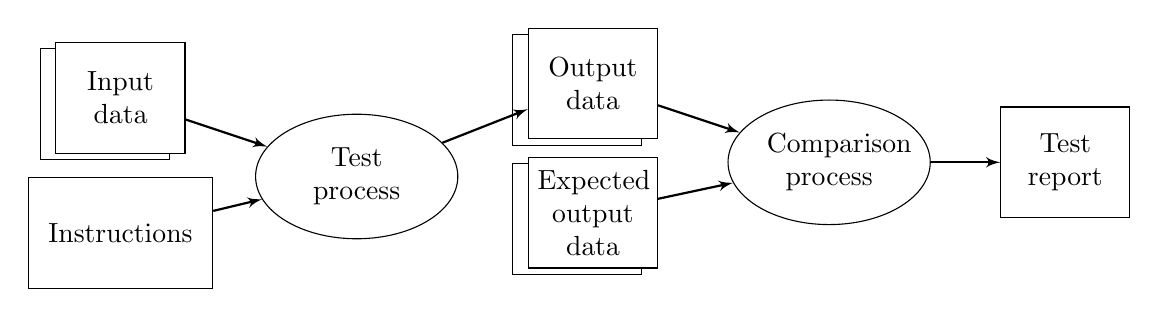
\begin{tikzpicture}[
    start chain=going below,    % General flow is top-to-bottom
    node distance=3mm and 30mm, % Global setup of box spacing
    ]
% ------------------------------------------------- 
\tikzset{
  base/.style={draw, on chain, on grid, align=center, minimum height=4ex},
  proc/.style={base, rectangle, minimum height=4em, text width=4em},
  proclong/.style={base, rectangle, minimum height=4em, minimum width=6em, text width=6em},
  elli/.style={base, ellipse, minimum height=4.5em, text width=4.5em},
  line/.style={draw, thick, -latex'}
}

\node [proc] (datain0) {};
\node [proc, fill=white, yshift=1.80cm, xshift=0.20cm] (datain) {Input data};
\node [proclong] (ins) {Instructions};

\node [elli, right=of datain, yshift=-1.00cm] (prc) {Test process};

\node [proc, right=of prc, xshift=-0.20cm, yshift=1.10cm] (dataout0) {};
\node [proc, yshift=1.80cm, xshift=0.20cm, fill=white] (dataout) {Output data};

\node [proc, xshift=-0.20cm] (exp0) {};
\node [proc, fill=white, yshift=1.80cm, xshift=0.20cm,] (exp) {Expected output data};

\node [elli, right=of dataout, yshift=-1.00cm] (com) {Comparison process};
\node [proc, right=of com] (rep) {Test report};

\path [line] (datain) -- (prc);
\path [line] (ins) -- (prc);
\path [line] (prc) -- (dataout);
\path [line] (dataout) -- (com);
\path [line] (exp) -- (com);
\path [line] (com) -- (rep);

\end{tikzpicture}
\caption{Automated integration test process adapted from \citet{fewster1999software}} \label{fig:autotestprocess}
\end{figure}

Each test is defined by the input data and instructions at the upper reaches of the process chain. The data should be complete enough for computational test execution. Comparisons are made with an array of different tools depending on the file format, though format support has come some way since Fewster's experiment.

The framework requires manual setup, for instance manual validation and storing of the expected outcome must be done before any tests can be automatically run. After some initial work, Fewster was able to squeeze out a 7 person-week reduction compared to manual testing \citep{fewster1999software}.

\section{Surrogate system}

\citeauthor{huang2008surrogate}'s \citeyearpar{huang2008surrogate} model, a precursor to the the same authors' unified testing framework presented in figure \ref{fig:liu}, is concerned with the testing environment arrangements related to stubs or mock services. The surrogate apparatus could be seen as a test harness and the tools for its construction. 

Figure \ref{fig:huang} already shows a clear framework structure stretching from test case generation to verification of system functionality. The area around simulating components is the area of focus, though both of the authors' models attempt to elaborate on the subprocesses and tasks that lie upstream on the testing process chain. \citep{huang2008surrogate}

\begin{comment}
\begin{figure}[H]
\centering
% =================================================
\pgfdeclarelayer{marx}
\pgfsetlayers{main,marx}
% -------------------------------------------------
% Start the picture
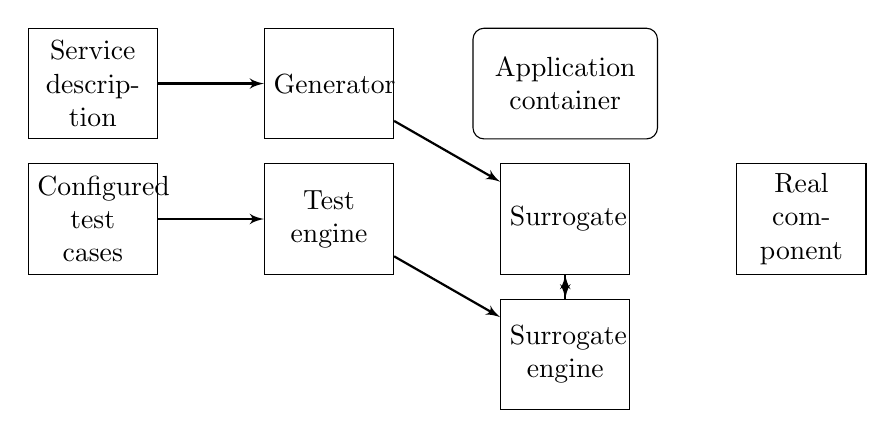
\begin{tikzpicture}[
    start chain=going below,    % General flow is top-to-bottom
    node distance=3mm and 30mm, % Global setup of box spacing
    ]
% ------------------------------------------------- 
\tikzset{
  base/.style={draw, on chain, on grid, align=center, minimum height=4ex},
  proc/.style={base, rectangle, minimum height=4em, text width=4em},
  cont/.style={base, rectangle, rounded corners, minimum height=4em, minimum width=6em, text width=6em},
  elli/.style={base, ellipse, minimum height=4.5em, text width=4.5em},
  line/.style={draw, thick, -latex'}
}
\node [proc] (desc) {Service description};
\node [proc] (tcs) {Configured test cases};
\node [proc, right=of desc] (gen) {Generator};
\node [proc] (ten) {Test engine};
\node [cont, right=of gen] (app) {Application container};
\node [proc] (sgt) {Surrogate};
\node [proc] (sen) {Surrogate engine};
\node [proc, right=of sgt] (rea) {Real component};
\path [line] (desc) -- (gen);
\path [line] (gen) -- (sgt);
\path [line] (tcs) -- (ten);
\path [line] (ten) -- (sen);
\path [line] (sgt) -- (sen);
\path [line] (sen) -- (sgt);
\end{tikzpicture}
\caption{Surrogate system architecture \citep{huang2008surrogate}} \label{fig:surrogate}
\end{figure}
\end{comment}

\begin{figure}[H]
  \begin{center}
    \includegraphics[width=13cm]{huang_et_al_framework.png}
    \caption{Surrogate apparatus architecture \citep{huang2008surrogate}}
    \label{fig:huang}
  \end{center}
\end{figure}

% The surrogate engine provides two kinds of technology independent interfaces: interface to configure component behaviour and interface to get simulated behaviour.

\begin{comment}
\begin{figure}[H]
  \begin{center}
    \includegraphics[width=13cm]{huang_testing_process.png}
    \caption{The testing processes by \citet{huang2008surrogate}}
    \label{fig:huangtesting} 
  \end{center}
\end{figure}
\end{comment}

In the surrogate apparatus, the environment is made of the application container which may or may not contain parts or the whole of the system under test and in which surrogate components, essentially mock services or stubs, are deployed. Again, the many interfaces in the framework are highlighted. The surrogate generator has a component for configuring surrogate components as well as a library of functions for imitated behaviour.

\citet{huang2008surrogate} instruct that before test execution the necessary surrogate components should be defined by test case and deployed. Before test case execution, the surrogate component availability is checked. To achieve true automation, then, such environmental setup should also be automated.

% data driven testing another way of saying automated testing?

\section{A unified testing framework}

The \citet{liu2009unified} model (Figure \ref{fig:liu}) includes processes, objects, and agents. Based on a UML sequence diagrams, the test generator semi-automatically creates test cases later submitted to the execution engine. Test runs are facilitated by a surrogate engine or engines which mock external systems. After execution, IBM's proprietary ITCAM technology aggregates execution traces together with the help of a trace correlator, which then pass the traces for transformation into a standard format. The test cycle is finished off by verification on the integration test case and execution trace and returning the result to the execution engine.

The surrogate \emph{generator} was conspicuously left out of the model. \citet{liu2009unified} chose to scope out this part of the framework and focus on the testing execution process rather than preconfiguration. The framework is dubbed 'unified' because it was designed to satisfy continuous integration testing requirements in a service-oriented environment.

The researchers separated test case structure and logic for platform independence. The test logic and configuration settings were encoded in separate XML files. The unified testing framework was built to be technology independent so 
separate plug-ins were created for the SOA context and technologies.

\begin{figure}[H]
  \begin{center}
    \includegraphics[width=13cm]{liu_et_al_framework.png}
    \caption{Unified testing framework \citep{liu2009unified}}
    \label{fig:liu}
  \end{center}
\end{figure}

The unified testing framework was tried out in relatively small-scale experiments, but successfully uncovered bugs early in development supporting the study's claims. The framework also helped find different kinds of bugs and didn't appear to have a bias towards uncovering a certain kind of defect \citep{liu2009unified}.

\section{Data-driven testing framework}

In \citeauthor{laukkanen2006data}'s \citeyearpar{laukkanen2006data} data and keyword driven testing model (figure \ref{fig:laukkanen}) testing is divided into modules for \emph{test design}, \emph{test execution}, and \emph{test monitoring}. A data-driven model, automation is enabled by correctly formatted and stored test inputs, test data, and driver scripts.

A test design system is used to create and edit tests cases. In practice, the system could simply be a spreadsheet or HTML editor. According to \citet{laukkanen2006data} the test monitoring system is used for controlling test execution and checking test results. The visualized results are in the form of low-level text logs or more visually-pleasing HTML.

At the heart of the framework lies the test execution system which houses test libraries, driver scripts, and the test data parsers, as well as the logger and report generator utilities. The monitoring system fires driver scripts which use functions in the test libraries and modules to perform test actions. The parser manages test data and converts to the right format. The logger collects relevant execution information which is also used as input in test reports. Both logs and reports can be viewed in the monitoring system. \citep{laukkanen2006data}

\begin{figure}[H]
  \begin{center}
    \includegraphics[width=13cm]{laukkanen_framework.png}
    \caption{\citeauthor{laukkanen2006data}'s \citeyearpar{laukkanen2006data} testing framework}
    \label{fig:laukkanen} 
  \end{center}
\end{figure}

Where the two first models essentially depict a loop and treat continuous testing as implicit, the keyword-driven model instead offers a monitoring step which overlays verification processes where a view to system status and health is more clearly separated from the testing execution. Naturally, a batch of test cases can be set to run to update the status. \citeauthor{laukkanen2006data}'s \citeyearpar{laukkanen2006data} model also supports the notion that a full framework should contain tools for the key processes test case generation, test execution, and verification (or monitoring).

\citet{laukkanen2006data} piloted the data and keyword driven framework in Windows application testing.

\section{Models summary}

The testing frameworks or models introduced in this chapter have striking similarities and subtle individual connotations. All models save for \citeauthor{huang2008surrogate}'s \citeyearpar{huang2008surrogate} surrogate architecture (only a part of the whole continuous integration process they later touch on) can be argued to follow a three step process of \emph{generating necessary input} (cases, surrogates, test data), \emph{running the test scripts}, and finally \emph{verifying and comparing results}. These three process funnels are comparable to e.g. \citeauthor{davenport1993process}'s \citeyearpar{davenport1993process} definition of a business process taking an input and producing a result or indeed a software method that takes some parameters and return some output.

% Alternatively: So as not to get too distracted by the rather pragmatic and technical models, a more holistic...
Since all of the models are rather pragmatic and technical, a more holistic perspective is reserved for further analysis of the nature of the integration testing framework. Figure \ref{fig:funnel} presents a framework on three levels of abstraction (horizontal dimension) in addition to the discussed process dimension (vertical). In doing so Figure \ref{fig:funnel} both sums up the presented models while putting them in a broader context.
%Pace of integration, rate of automation, definition for I/O process

\begin{figure}[H]
\centering
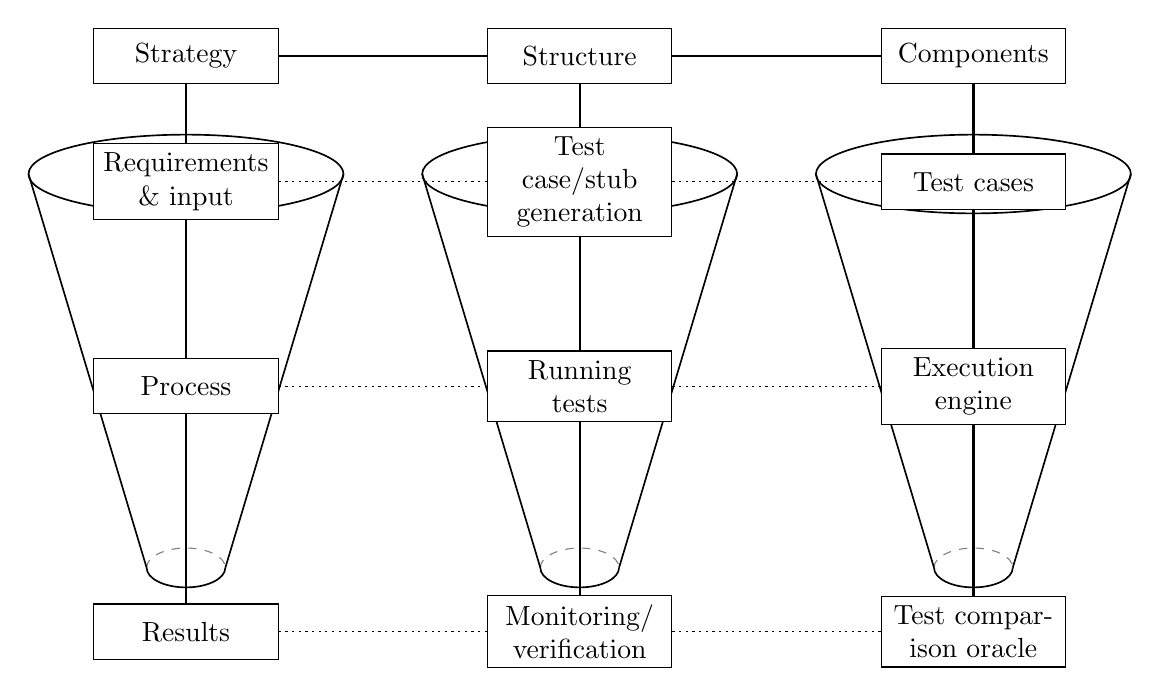
\begin{tikzpicture} [ 
   start chain=going below,         % General flow is top-to-bottom
    node distance=10mm and 50mm,    % Global setup of box spacing
    ]
% ------------------------------------------------- 
\tikzset{
  base/.style={draw, on chain, on grid, align=center, minimum height=4ex},
  rect/.style={base, rectangle, minimum height=2em, text width=6em},
  line/.style={draw, thick}, %, -latex'},
  dots/.style={draw, dotted} %, -latex'}
}

    \draw[semithick] (-5,0) arc (180:0:2 and 0.5);                  % cone 1: top ellipse top arc
    \draw[dashed,color=gray] (-3.5,-5) arc (180:0:0.5 and 0.25);    % cone 1: bottom ellipse top arc
    \draw[semithick] (-3.5,-5) arc (-180:0:0.5 and 0.25);           % cone 1: bottom ellipse bottom arc
    \draw[semithick] (-5,0) arc (-180:0:2 and 0.5);                 % cone 1: top ellipse bottom arc
    \draw[semithick] (-5,0) -- (-3.50,-5);                          % cone 1: left side
    \draw[semithick] (-1,0) -- (-2.50,-5);                          % cone 1: right side
    
    \draw[semithick] (0,0) arc (180:0:2 and 0.5);                   % cone 2: top ellipse top arc
    \draw[dashed, color=gray] (1.5,-5) arc (180:0:0.5 and 0.25);    % cone 2: bottom ellipse top arc
    \draw[semithick] (1.5,-5) arc (-180:0:0.5 and 0.25);            % cone 2: bottom ellipse bottom arc
    \draw[semithick] (0,0) arc (-180:0:2 and 0.5);                  % cone 2: top ellipse bottom arc
    \draw[semithick] (0,0) -- (1.5,-5);                             % cone 2: left side
    \draw[semithick] (4,0) -- (2.5,-5);                             % cone 2: right side

    \draw[semithick] (5,0) arc (180:0:2 and 0.5);                   % cone 3: top ellipse top arc
    \draw[dashed, color=gray] (6.5,-5) arc (180:0:0.5 and 0.25);    % cone 3: bottom ellipse top arc
    \draw[semithick] (6.5,-5) arc (-180:0:0.5 and 0.25);            % cone 3: bottom ellipse bottom arc
    \draw[semithick] (5,0) arc (-180:0:2 and 0.5);                  % cone 3: top ellipse bottom arc
    \draw[semithick] (5,0) -- (6.5,-5);                             % cone 3: left side
    \draw[semithick] (9,0) -- (7.5,-5);                             % cone 3: right side

    \node [rect, xshift=-3.0cm, yshift=1.5cm, fill=white] (stg) {Strategy};
    \node [rect, yshift=0.25cm, fill=white] (req) {Requirements \& input};
    \node [rect, yshift=-0.75cm, fill=white] (prc) {Process};
    \node [rect, yshift=-1.4cm, fill=white] (rlt) {Results};
    
    \node [rect, right=of stg, fill=white] (fmw) {Structure};
    \node [rect, right=of req, fill=white] (tcg) {Test case/stub generation};
    \node [rect, right=of prc, fill=white] (run) {Running tests};
    \node [rect, right=of rlt, fill=white] (mon) {Monitoring/ verification};
    
    \node [rect, right=of fmw, fill=white] (art) {Components};
    \node [rect, right=of tcg, fill=white] (tcs) {Test cases};
    \node [rect, right=of run, fill=white] (exe) {Execution engine};
    \node [rect, right=of mon, fill=white] (out) {Test comparison oracle};
    
   % \node [rect, below=of mon, yshift=-1.0cm, fill=white] (pit) {Pitfalls};
     
    \path [line] (stg) -- (fmw);
    \path [line] (fmw) -- (stg);
    \path [line] (fmw) -- (art);
    \path [line] (art) -- (fmw);
    
    \path [line] (stg) -- (req);
    \path [line] (req) -- (prc);
    \path [line] (prc) -- (rlt);
    
    \path [line] (art) -- (tcs);
    \path [line] (tcs) -- (exe);
    \path [line] (exe) -- (out);
    
    \path [line] (fmw) -- (tcg);
    \path [line] (tcg) -- (run);
    \path [line] (run) -- (mon);
    
    \path [dots] (run) -- (prc);
    \path [dots] (prc) -- (run);
    \path [dots] (run) -- (exe);
    \path [dots] (exe) -- (run);
    
    \path [dots] (req) -- (tcg);
    \path [dots] (tcg) -- (req);
    \path [dots] (tcg) -- (tcs);
    \path [dots] (tcs) -- (tcg);
    
    \path [dots] (rlt) -- (mon);
    \path [dots] (mon) -- (rlt);
    \path [dots] (mon) -- (out);
    \path [dots] (out) -- (mon);
 
\end{tikzpicture}
\caption{Process levels in integration testing} \label{fig:funnel}
\end{figure}
%remove arrows?

The framework is divided into strategic, technical/structural, and component levels. Starting from the left the framework becomes more and more fleshed out. First, the general testing \emph{strategy} and requirements are accepted as premises and translated into a framework \emph{structure}, largely uniform, but flexible enough to conform to minor project idiosyncrasies. In each separate case framework scope is outlined by specifications and agreements e.g. on security policy or service level, and more formally described in a test plan, which typically includes test objectives, responsibilities and schedules, a list of necessary tools, process descriptions, and success criteria \citep{myers1976software}.

The structure should be robust or modular enough to be separable into clear and concrete constituent \emph{components}, like test cases, in human or machine readable form. These should be constructed with regard to the framework strategy and structure scope. The modularity permits the fluent addition of new test cases, integrations, or other components to the framework.

It should be remarked that the models do not address performance testing directly. Perhaps the model creators reasoned this was implicit in the frameworks, automation being the key enabler for load and stress tests. It all boils down to which measures should be followed. If the \emph{execution traces} include relevant metrics then performance testing is logically possible through the framework.

\begin{comment}
The testing process can vary in its mode of execution or degree of automation. In what is perhaps the most extreme case, test case are run automatically every time a change is committed to system source code. This approach is called continuous integration (CI). 
\end{comment}

% add test harness to surrogate introduction

\chapter{Deconstructing the framework}
\label{chapter:frameworkanalysis}

% drop something in funnel runs automatically 
This chapter examines individual components and subprocesses of integration testing, based on topic areas highlighted by the models and model synthesis derived in the previous chapter. Essentially, we traverse \ref{fig:funnel} one box at a time, from strategy to components, and from test requirements to the test comparison oracle. 

The first section enumerates important testing strategy decisions, while the next concentrates on practical questions and what options and tools there are to implement the strategy and structure the framework. The third section evaluates the framework from a component and maintenance perspective. Finally, we take step back and take heed from potential testing and automation pitfalls presented in academic literature. The desired outcome of the deconstruction is to have the understanding necessary to assemble a whole new framework tailored for the case company's needs.

\section{Testing strategy}

Testing strategy is broken down to aspects of coverage-efficiency requirements, process design, and how test results are used to drive quality and further improve testing practices. More precisely, the first strategy choice is test case selection and design, the second the test control and management model, and the last test and framework improvement through feedback.

\subsection{Requirements for coverage and efficiency}

One can observe that because testing must only provide reasonable confidence in system performance, it can be selective. Not everything should or indeed can be tested. Focusing on a part of the whole system saves time and costs. It is however essential to model and understand the system flow and which part of it should be tested. If only a part of system is known to have changed, testing can be limited to the new functionality \citep{bhuyan2012survey}. Similarly, effort put to test case production should be defined by planning coverage and case selection. Ideally, the set of cases provides minimum required coverage based on testing strategy and business strategy criteria. 

% test types to glossary?
When tests compare as much information as possible, they are called sensitive tests. Conversely, more selective comparisons constitute robust tests. Both of the test types can be useful in different stages of testing. Sensitive cases are likely to require more maintenance and updating, but provide more accurate information about the results and are less likely to miss defects. A good automation testing strategy utilizes both in a way which avoids redundant testing, but at the same time provides adequate coverage. \citep{fewster1999software}

Overall test effectiveness can be measured by how many cases were executed out of the set of necessary cases and feature testability by how many test cases are necessary for satisfying a criterion \citep{linnenkugel1990test}. Therefore attention must be spent on both selecting the method of execution, and test criteria. 

The most common way to evaluate coverage is based on control flow, which simply means the order in which individual statements, instructions or function calls occur. Visualizing the program process flows can help understand the program logic, potential features to test, and guide the construction of test cases, too. \citep{burnstein2003practical} 

\citet{linnenkugel1990test} present a flow-oriented coverage hierarchy of node, relation, call, sequence, and loop coverage measures. For integration testing, individual components (modules) are nodes and integrations are relations (call statements). \citeauthor{linnenkugel1990test}'s \citeyearpar{linnenkugel1990test} coverage criteria include:
\begin{itemize}
\item \emph{all-modules} requires that every module is executed at least once 
\item \emph{all-relations} requires that the calling relation between modules is executed at least once
\item \emph{all-multiple-relations} requires that every call between modules is executed at least once
\item \emph{all-simple-call-sequences} requires that every sequence of (descending) calls without repetition of calls is executed at least once
\item \emph{all-call-sequences} requires that every sequence of (descending) calls is executed at least once
\end{itemize}
Here, complex path sequences can be interpreted as system tests, whereas \emph{all-relations} and \emph{all-multiple-relations} fall under integration testing. The first item requires that each software module works, the second that at least one of the services between modules is tested, the third requirement is that all possible exchanges between two connected modules are tested, the fourth requirement includes all end-to-end execution paths without repetition or loops, and lastly end-to-end tests which may contain loops.

\citet{hewett2009automated} persuade testers to lay out and quantify components and their connections in a graph and use this information to minimize the need for creating test stubs and design the most efficient order for testing. Likewise, \citet{leung1990study} and \citet{abdullah1995correcting} endorse the concept of a firewall which draws a line between components and systems that are to be tested, and those that aren't. The divison is based on where changes in code or specifications have occurred. This modelling both strengthens understanding of the inner workings of the tested system and reduces testing costs.

In particular researchers advocate the creation of a call graph \citep{leung1990study, hurlburt2012not, linnenkugel1990test}, which explicitly maps interactions and relationships between integrated system components. The graph can serve as a foundation for organizing testing and setting test coverage criteria and strategy or test case creation \citep{benz2007combining, hura2011method, linnenkugel1990test}. In practice, a systematic testing sweep can be based on e.g. some of \citeauthor{linnenkugel1990test}'s \citeyearpar{linnenkugel1990test} coverage criteria. 

Deriving test cases from models or using models to represent the testing strategy is known as model-based testing and uses specifications or program code to first derive the model \citep{pezze2008software}. An accurate model has the benefit of reducing specification errors and misinterpretation by providing a common point of reference. Using model-driven integration \citet{wieczorek2010model} estimated savings of 50\% in time for test generation and concretization tasks.

A model can be used to implement automated testing or test case creation, and elicit possible execution paths and plan coverage, and ensure that the system is adequately tested. For instance, a finite-state machine is a formal model which is depicts sequences of interactions between system components. Some systems, like those in banking and medicine, have very high availability requirements and therefore take advantage of formal models for comprehensive testing and significantly reduced risk. Models can also be less formal, for instance class diagrams or even constructed from documentation that is composed entirely of natural language. \citep{pezze2008software}

\subsection{Choosing the integration test process}
The way integration testing is conducted is linked to the integration strategy. Service-Oriented Architecture and Continuous Integration especially blur the line between development and integration \citep{huang2008surrogate, wieczorek2010model}.

\citet{myers1976software} introduces six integration strategies: bottom-up, top-down, modified top-down, sandwich, modified sandwich, and big-bang testing. Each strategy influences the form in which test cases are written, the types of tools needed, the order in which separate components are coded, and the thoroughness and economics of the testing effort. 

In \emph{bottom-up} and \emph{top-down testing} integrations are put together and tested one by one, starting from either low-level systems --- or the top-level systems that are not called by any other system. Both approaches require mock systems to simulate integrations, either just below or above the tested system component. In \emph{big-bang testing}, the integration testing effort is delayed until the system is wholly ready and put together. Each component is unit tested before the eponymous big-bang. \emph{Sandwich testing} is a combination of top-down and bottom-up testing where two concurrent testing threads progress towards the middle layers of the system. If it were better that some of the middle layers were tested first, the approach can be modified accordingly. \citep{burnstein2003practical, myers1976software}

\citet{pezze2008software} point out that big-bang essentially merges integration testing with system testing. While it reduces costs of 'test scaffolding', the structure (e.g. stubs and drivers) needed to carry out piecemeal testing, a delay in testing is not ideal for a large and complex integration undertaking. Examining the integration as a whole and pinpointing defects is difficult in the tumult of the big-bang \citep{myers1976software, pezze2008software}. A better option would be to test early and little by little. This is as much a development strategy as a testing strategy. % with referene to BDD and TDD

% literature development minded, regressions tests when systems are already put together, comes down to order of testing, but tests can be executed instantaneously. how realistic, how sophisticated, coverage of links
The strategy typology is designed for integration in the development phase, rather than integration regression testing, which limits its applicability. An automatically executable test set may be capable of going through every integration in a matter of seconds or minutes, especially if only a few integrations are tested at a time. This makes the question of order (e.g. top-down or bottom-up) rather moot. The strategies, however, are worth considering when changes in systems call for testing many integrations (possibly all of them), for example when reassembling the system is required after a change with global effects. Integrations that are quick to run, or likely to fail should be run first \citep{duvall2007continuous} 

%Theoretical number of states infinite 
% Guide slection, specs are lacking, is the fsm feasible
% The more formal the model, the better test cases, still support (pezze). 
% Criticize avoiding bigbang
%While continuous testing has been advocated since a long time \citep{myers1976software}, it has also found home in %more recent software development trends, like eXtreme Programming and Agile (reference).
%
% Extreme Programming Explained: Embrace Change (Addison-Wesley, 1999)
%
% Continuous testing, continuous integration, test-driven development
% duvall: realiability at the lowest level
%
% What are the methods of execution? (not technical, move to framework section in the automation part)
% How are results used?
%
% regression strategy, code-based: cases selected to account for changed code, pezze 428 specification-based criteria select a test case for execution if it is relevant to a portion of the specification that has been changed. fault proneness, random sampling, priorities (recent has low), fault-based, coverage+age

\subsection{Using test results}
The purpose of testing is to reveal bugs in the software \citep{burnstein2003practical}. But this is a rather narrow-minded view. The testing framework should deliver results so that they can help developers fix the found defects. As such, though, defect management is not in the scope of the testing framework. In Wärtsilä's case there already is a bug tracker tool in use and logging new defects is left to human discretion and manual work. The framework should, however, record test execution times, system version numbers, and other contextual metadata so that testers can manage system releases and defects \citep{jenkins2008software}.

Testing results can be used to evaluate and analyze the testing process and framework. \citet{jenkins2008software} advocates measuring found defects\footnote{Only those that have been confirmed as defects and have not been rejected.} per tester work hours, or how well are new issues are discovered, to determine if testing efficiency. Ideally, this figure would be compared to manual testing figures. \citep{jenkins2008software, fewster1999software} To evaluate integration testing in particular one might also measure defect detection as a percentage, i.e. defects found at a stage in testing divided by all known defects. Naturally, the figure can only be calculated after all testing. The thesis does not delve into which metrics are best. Indicators should be evaluated according to Wärtsilä testing policy.

While this thesis does not assert how results should be used in decision-making as such, results can also guide further testing efforts. In \emph{fault-based testing}, new test cases (and more strict specifications) are designed for each problem areas, which are then more heavily tested. \citep{pezze2008software} The framework is improved iteration after iteration. In a similar vein, once the test cases have been created and chosen, the test set quality itself can be evaluated quantitatively and 'tested' based on test results. For example, in \citeauthor{delamaro2001interface}'s \citeyearpar{delamaro2001interface} \emph{mutation testing} the test set quality is evaluated by creating variations of the tested programs and running the cases against the mutated programs. If a case passes against the mutated program, it is considered \emph{live}. Ideally, cases will fail when run against modified, 'erroneous' code. 

\section{Framework structure}

This section examines the framework-object relationships and structure. First, test case design and generation, then test execution, and finally verification or validation are covered. The purpose is to draw on academic writings and experiments for establishing the basic structure of the testing framework, to get acquainted with related techniques that have been put to use previously, and identify any other practical concerns in designing a successful testing process.

\subsection{Test case generation}

% meyer: case extraction out of failures, alternative test generation strategies
Test case creation is perhaps the most time-consuming task in automated testing \citep{kit1999integrated}. Cases have to be produced based on the test plan and execution strategy and updated when necessary. Researchers and testing engineers have presented different solutions for automatic test case generation, but all in all two major possibilities exist for automatically generating test cases: model-based approaches --- and recording or capture.

Models or contracts derived from code or system specifications can be used to create test cases. \citet{tsai2002coyote} introduces an XML-based framework for automated test case generation from WSDL service descriptions. \citet{bai2005WSDL} and \citet{di2007web} similarly offer WSDL service description based generation strategies. \citet{dalal1999model} present a combinatorics-based data model that produces a minimum number of test cases for some input parameter related coverage criteria. Formal models, like finite state machines, can also be used to produce test cases, though the formalization of vague specifications and constructing the model in such a way that test case production is possible takes time and effort, and can make model-based approaches look unattractive compared to the alternative, capture and replay. 

In situations where the system suite is already in place, cases and related test data can be produced by recording or capturing user actions in the system environment and turning these into use cases that can be automatically replayed. However, researchers like \citet{zallar2001you} and \citet{kit1999integrated} criticize the capture/replay paradigm claiming that maintaining the test scripts is cumbersome and will often be left undone rendering the test cases unusable and potentially misleading. \citet{kit1999integrated} suggests to just leave out capture and simply use automation to replay. \citet{pezze2008software} confirm that repetitive tasks should be automated --- not creative ones. \citet{fewster1999software} also bluntly state that \emph{"record and replay is not test automation"} though their message is that there is more to testing, and that record/replay still requires manual work to achieve automation. 

\subsection{Running automated tests}

The testing process is performed by an engine program that runs the test cases. Tests can be scheduled to run at regular intervals or they can be triggered by developer actions, such as a code commit \citep{pezze2008software}. Continuous integration (CI) is a development philosophy where integration is reduced to a "nonevent" by integrating new code with old as soon as the former is ready. All tests must pass for the build to be accepted. \citep{duvall2007continuous} The risky big-bang is thus avoided.

While extreme, CI's continuous testing can make integration more manageable with its gradual approach. In the case of integration testing, the important execution decisions are related to integration strategy, i.e. which tests run first \citep{duvall2007continuous}. If test cases have been prepared, regularly rerunning tests and regression testing is easy, though implementing automated test processes still takes an initial investment of time and effort. Additional automation issues are examined in Section \ref{section:pitfalls}.

The most sophisticated execution methods include data and keyword-driven testing. The first means that script logic is separated from input data so that the same script can be reused because the input payload is not configured into each case. Keyword-driven testing is very complicated in involves creating a layer of abstractions so that test scripts can be written using predefined keywords which act as functions 

The technical automated execution challenge is not as interesting as test case generation or oracle construction because scheduling is simply a technical requirement. Most operating systems can run commands or scripts at specified times. Accordingly, more attention is paid to the latter topics. It should be noted that execution is a de facto feature of development environments where test resources, like cases, are created. Selecting this tool or technology is an important issue, which depends on the tool's additional features as well as other contextual factors, but will not be explored here.

\subsection{Verification}

Verification is the step that applies value to test execution. It transforms data from test runs to information with meaning. It is the culmination point of testing. Verification can be done ad hoc and manually, but here we examine the topic from the point of view of frameworks and testing tool and automation \citep{fewster1999software}.

Colloquially, the step is often associated with \emph{test oracles} which analyse results and apply pass/fail criteria to determine if a test was successful or not \citep{pezze2008software, burnstein2003practical}. Oracles determine success and failure by comparing program output to expectations. These comparison-based oracles are an essential part of testing frameworks and test harnesses. \citep{pezze2008software}

Rather than talk about some revered oracles \citet{fewster1999software} argue for the term 'comparison' since automated algorithms cannot assert success of failure, but only apply predefined rules to the test outcomes. It remains the test engineer's responsibility to discern between success and failure; to the machine truth is just bits. Because comparison is a repetitive task requiring great attention detail and involves comparing digital, often explicit outputs in standard form (like XML), it is ideally suited to be automated. \citep{fewster1999software}

\citet{fewster1999software} also make a distinction between dynamic and post-execution comparisons. In the former, pass/fail rules are applied automatically as the cases are run. In the latter, the collected execution traces are subjected to a comparison engine after the execution. Sometimes the distinction is less obvious, for instance when a comparator evaluates output after case execution but during the overall test run. It is largely an architectural question of where comparison logic should be stored. Some degree of verification during the run is advantageous as it can flag errors in the test configuration and abort a test run that would not provide any useful results \citep{fewster1999software}.

Comparison also differs in complexity. Simple comparison looks for an identical match between output and expected output. The approach is effective but inflexible. Complex comparison takes into account known variance in test results. Testers also need to define the granularity of test scripts, or how many comparisons are made. Having many comparisons makes for more high quality test cases but also increases their upkeep and creation costs \citep{fewster1999software}. 

Defining expected results naturally means more work in test case creation. There are options to mitigate this, for example by using 'correct' output from previous versions of the system or a trusted alternative to the one tested. One can see that the oracle/comparator question is already present in case generation, for example when cases are first captured and created the output can be stored as expected outcomes. This first verification must be done manually before the test cases are stored for automated execution (\citet{fewster1999software} call this 'reference testing') In the most ambitious method, program execution is documented in a specification model in the full, so that the model can be used to both generate test cases and used as an oracle. \citep{pezze2008software}

\section{Framework components in operation}

As new integrations are introduced, old ones go through changes, or some other trigger for testing occurs, the framework should provide a test harness that is easy to adopt. Integration test cases should have a template and their addition to the automatically executed test packages should involve a reasonable amount of work \citep{fewster1999software}. The case creation guidelines, especially when paired with capture techniques, can expedite the testing process when compared to ad hoc testing and add the security of control. All this procedure related to automated testing adds to the software maintenance costs. It is therefore essential to evaluate and discuss what the continued use of a testing framework would entail.

\subsection{Test case management}
% add mock service
Test cases encompass requisite input information, script logic, and expected outcome for the execution of tests. The cases are the arrows in the quiver of the tester. Along with mock services or surrogates, they are strategic resources in that they determine the effectiveness of testing, but their creation, as well as maintenance, is also an investment.

With an automated framework, one might be tempted to add more and more cases for "increased confidence in the SUT" especially when execution only takes seconds. This is a common error of judgement \citep{fewster1999software}. The amount of cases should be as small as possible for the least possible amount of maintenance work including test set-up and clean-up tasks. Tests should not overlap, or test the same features and functionalities, and they should contain as little script code as possible. To remedy the situation, \citet{fewster1999software} recommend reviewing new test cases before they are accepted and periodically weeding out less important cases. 

On the other side of the coin, dividing cases into a fine level of granularity is justified, too. Brief, focused cases enable quick and efficient test runs and to discern where exactly the bug is. The analysis of bugs after discovery takes up a significant amount of time and resources. Accordingly, there is no universal truth to what the best amount of test cases is.

\citet{fewster1999software} report that developers and testers typically spend two minutes looking for a suitable test resource before giving up and making one themselves. This poses a threat to the testing framework: duplicate resources, work, and ignoring the framework architecture and rules of use to name just the obvious. The first test case management challenge is that test resources (cases and e.g. surrogate components) should be stored in a centralized library which enables finding cases easily. Therefore, tests should be supplemented with comments and descriptions of their purpose to afford searches in the library.

The test resource library can also house related documents and records produced during tests. As these can quickly clog up a data base, most by-products from successful runs are deleted, but some records of test success and failure should be saved and used as steering metrics. \citep{fewster1999software} To manage the limited storage space test case developers should be provided with instructions as how, and in which format, to store test data. The format choice must be balanced between simplicity and understandability (for both man and machine), and flexibility and ease of use.

% commercial tools usually dynamci
% not too many complex cases
% support, automated updates to test data and define standards and values
%  add to conclusion: figure out most importnat automation concerns and focus on them

As for test case logic structure, \citet{duvall2007continuous} recommends including only one assertion per case so that final results can easily be traced back to the underlying problem, though \citet{fewster1999software} write that some features require multiple checks to verify (e.g. inserting data into a database).\footnote{One case might also be divided into multiple "subcases" each with their assertion.} Test case scripts can be designed so that they take into account certain circumstances and adjust to their conditions intelligently \citep{fewster1999software}, for instance reacting to a severed network connection. The added dynamic script logic bloats the cases and makes them more cumbersome to maintain, though. As reruns rack up the testing time, test execution time should be as quick as possible. If something is clearly wrong the run should stop so no time is wasted.

Whenever changes are made to a feature in software, test cases should also be updated accordingly or in some cases it makes sense to create a new case entirely. Uniform structure, centralized storage, and metainformation can already facilitate this process. Of course left unattended, the deprecated cases may well fail prompting the update task where needed, but they might also claim success while leaving something new and important out of the test scope.

% todo, much depends on the used framework
% Summary: Many tradeoffs, test manger responsible.
% switching to another tool
% Tracker a separate tool. Test case id communicable, can be run individually.
% pre and post processing, e.g. setting up env and delting by products

\subsection{Running the engine}

The execution engine is essentially the tool selected to run test cases. It is integrated and configured to the development environment or test resources. The maintenance and daily use issues boil down to cost of the product, availability in the target organization, and ease of use and support. As the development environment allows for test runs it usually also presents the outcome of such runs and can serve many purposes. Naturally, other tools can be brought in to handle test runs or verification, or presenting test results.

Cost should be compared to benefits from test automation and any alternative tools. It should also be estimated how easy it would be switch from one tool engine to another should the need arise (e.g. avoiding vendor lock-in). This is also why test resources should be stored in a standard rather than proprietary format.

Second, the test manager must make sure everyone who needs the tools to create test cases or surrogate components has the means to do so. Availability might be bottlenecked by licensing or hardware concerns. Of course, in reality it might be that cases are constructed centralized by a test engineer rather than software application or service experts.

Finally, everyone who uses the execution engine must know how to do so. This is not just a task for the framework administrator but for anyone who contributes resources to the framework, though the mains responsibility of drawing up instructions does befall on the testing experts. As for support, a little work upstream avoids build-ups of work at the downstream caused by negligence of correct practice.

\subsection{Maintainable comparison} 

Test comparison can be very detailed, or filter out irrelevant execution traces and only verify a portion of the results. The format of data is important both in terms of efficient storage and easy processing. Standard formats, like XML, are best suited for comparison.

\citet{fewster1999software} present a helpful checklist for implementing a maintainable comparator:
\begin{enumerate}
\item Remember that matching outcomes to previous outcomes is tricky. Dates and timestamps change.
\item Document comparisons so whoever uses them understands what they do.
\item Agree on and adhere to sensible naming conventions.
\item Keep comparisons simple to make updates and changes easier to do. 
\item For complicated or lengthy comparisons think if they can be simplified, or if manual comparison would make more sense.
\item Standardize to create reusable building blocks for constructing the comparison logic statements (e.g. reusable filters and regular expressions).
\item Use a balanced mix of sensitive and robust comparisons. If required by testing objectives, create different test cases for the two so they can be run separately.
\item Divide and conquer: create separate comparisons for each feature for easy set-up and matching to testing need.
\end{enumerate}

There is a degree of contradiction in the guidelines, for instance creating and maintaining a reusable logic statement library while keeping the method of comparison approachable and easy to maintain. \citet{fewster1999software}'s advice is still compelling if the development effort is big and new features are continuously added.

\section{Integration testing pitfalls}
\label{section:pitfalls}

Testing management is no light matter: \citet{reid2005art} evaluated that about 50\% of system development time and more than 50\% of costs are spent on testing. A relatively small mistake can be costly and, indeed, integration testing can fail in many ways \citep{van2008identifying}. This section takes stock of the most common pitfalls in both testing and integrations.

Testing may be overlooked as a non-value-adding activity and integration considered \emph{done} as soon as systems have been connected. Alternatively, testing resources are considered expendable, and testing given a low priority, reducing it to a project's \emph{'crushable zone'}. According to \citet{van2008identifying}, not identifying and communicating integration strategy, responsibilities and accountabilities, lines of reporting and escalation --- or sharing knowledge --- are also typical pitfalls, exacerbated by lack of expertise and good document management. Additional problems are caused by physically separated locations, and failing configuration or incident management. \citep{van2008identifying}.

There are also many potential stumbling blocks in automation. Algorithms cannot match the intelligence and intuition of an experienced human tester and \citet{kaner1997pitfalls} points out that automated tests cases are usually simple in structure and consequently less likely to stumble upon a bug. Some systems undergo so many changes that automation makes little sense: as these changes are introduced into the systems and code, related test cases must be examined, their reusability ascertained, out-of-date cases should be discarded, and new cases created where necessary \citep{zhang2011approach, kaner1997pitfalls}. Automation does not counteract inherently flawed software development or testing processes. \citep{jenkins2008software, zhang2011approach).

\citet{kaner1997pitfalls} reminds that automation takes time and can slow testing down at first. The typical implementation workflow is to first execute a test case manually to see that it passes and then automate it. This results in an effete set of test cases which finds bugs at reduced rate compared to manual testing \citep{kaner1997pitfalls}. Adding too many cases makes testing counterproductive because of difficult and expensive maintenance.

\citet{leung1990study} present a typology of integration errors and classify them to interpretation errors, interface errors and miscoded call errors, which are again divided into subgroups. Errors may be the result of superfluous, missing, or plainly incorrect function calls. These can be further mapped under interpretation errors which are mistakes in program logic, miscoded error calls where the functionality happens at the wrong time or place, or interface errors where standards and agreements have been broken. The error types are presented in figure \ref{fig:errors}.

\begin{figure}[H]
\begin{center}
    \begin{tabular}{ l || >{\raggedright}p{3cm} | >{\raggedright}p{3cm} | >{\raggedright\arraybackslash}p{3cm} }
      & Interpretation error & Miscoded call error & Interface error \\ \hline \hline
    Wrong & Incorrect functionality & Call instruction at wrong location on path & Standards or agreements are violated \\ \hline
    Missing & Not all necessary functionality implemented & Call instruction missing on path & Standards or agreements are violated \\ 
    \hline
    Extra & Function performs more than what is expected or needed & Call instruction on a path which should not have it & Standards or agreements are violated \\
    \end{tabular} 
\end{center}
\caption{Integration testing errors, adapted from \citet{leung1990study}} \label{fig:errors}
\end{figure}

% to avoid miscoded error call test test cases
% to avoid standard violations test test cases
% to avoid intepretation error focus on specification, test 

A testing framework can serve to define common ways of working and alleviate the testing time crunch by speeding up testing through automation. It cannot answer problems in communication of responsibilities and accountabilities, though it can offer a shared view into test results and the current state of the SUT.  

While the testing tool cannot prevent the errors listed in Figure \ref{fig:errors} it is equipped to detect them quickly and make records of each one. Studying bugs has its merits. Determining which kinds of errors are most common and testing for them in particular is known as fault-based testing. It has been found quite promising but is not yet widely applied in the field of software testing. \citep{pezze2008software} Ideally, a test framework will collect information about execution so that defect analysis is possible. This can point to ways to improve integration quality and lighten the burden on testing.
  
\chapter{Piecing together a new framework}
\label{chapter:frameworkproposal}

In Chapter \ref{chapter:frameworktheory} \citet{fewster1999software}, \citet{huang2008surrogate}, \citet{liu2009unified}, and \citet{laukkanen2006data} presented framework models for integration testing, the key processes of which include test case generation and design, executing test cases, creating mock systems, simulating unavailable systems or services, verification of results, and execution monitoring. Chapter \ref{chapter:frameworkanalysis} further distilled the essence of an automated test framework into individual elements. This chapter takes these building blocks and, according to instructions laid out already in Chapter \ref{chapter:background}, assembles a framework suitable for Wärtsilä. 

The presented model is paired up with a technical implementation proposition or construct. The purpose of the construct is to act as proof of concept and, in true testing style, give early indicators of how valid the theoretical foundations are. The proof of concept is also ideal in highlighting practical concerns that can only arise in a live test.
%After a framework model is shown, the chapter continues to practical implementation and showcases a construct built %to address Wärtsilä's testing needs which were documented in Section \ref{section:requirements} and based on theoretical observations made earlier in Chapter \ref{chapter:frameworktheory}. 

\section{Wärtsilä's integration testing framework}

The framework constructred for Wärtsilä synthesizes and combines integration testing theories and techniques introduced in Chapter \ref{chapter:frameworkanalysis}. The model is perhaps most inspired by the \citet{liu2009unified} unified testing framework model, but adapted to Wärtsilä's integration testing needs. As such, it is technology-agnostic, and only presents the steps, systems, system-document relationships, and processes required on an abstract level. The framework hypothesis is presented in Figure \ref{fig:framework}.

\begin{figure}[H]
\centering
\includegraphics[angle=90,width=12cm]{framework.png}
\caption{Original testing framework hypothesis}
\label{fig:framework}
\end{figure}

There are a total of six processes and three objects involved in the proposed framework, along with the system under test (SUT) and a test resource database. The processes are divided into two steps. The first, preparatory step, contains the creation and preparation of test resources while in the second, the execution step, those resources are exercised in conducting integration tests. The execution step repeats itself, depending on how the tests should be scheduled.

% assertions
In the preparation step a new test resource, that is to say a test case \emph{or} a mock service, is created first by capturing message records, and secondly using these to generate the desired test resource. Consequently, 
the selected testing tool(s) must support recording messages and the generation process. Before being added to the test resource database, created cases and surrogates are put through the execution step to make sure they work without error and are suitable for automation. When cases or mock services are ready they are run and verified before being saved as test resources in the appropriate files or packages in the test database. This concludes the pre-test setup work. The actual testing begins when scheduled test runs pick up cases or invoke mock services and they go through the testing step again.

The generation process is likely the most labour-consuming and must be planned and supported by clear documentation and accessibility to necessary tools and documents. It should also be noted that the generation step is not entirely automatic, and the tester must specify which messages are used for test resource generation and which parts of the system communication is examined in the verification step. (In other words, the test oracle is configured in each test case.) The configuration involves the creation of assertions, or explicit logical expressions of the expected outcome, which can be computationally executed. 

Since there are cases where correct system behaviour cannot be verified by examining an output, service mocking is required. Consequently, a framework also needs a component for the creation of such mock-ups, preferably using a strategy similar to the one in test case creation; actual records from production can be used as basis for mock service emulation.

Theoretically, models, diagrams, and specifications can also be used for automatically producing test cases, but the reality at Wärtsilä is that these are not documented in such detail that would practically afford such generation. At least, models and specifications should be used to make sure the test cases address and measure correct things and defined behaviour, and to communicate system structure and logic. 

The framework enables automated integration testing by scheduling test runs. Each run picks up a set of test cases which it then takes through the execution step. First, a testing tool runs the cases and collects execution traces as they are produced. The traces are used in the verification process and compared to expected results to determine if a case has failed or not. Finally, the results are logged in the test database.

% A surrogate engine refers to any scheme which is employed to act as a stand-in for unavailable, or testingwise unsuitable, systems. The surrogate engine's role is particularly important in the development phase, when not all components are fully ready.
\begin{comment}
\begin{figure}[H]
\centering
% =================================================
\pgfdeclarelayer{marx}
\pgfsetlayers{main,marx}
\xdefinecolor{lightgrey}{RGB}{220,220,220}
\xdefinecolor{blackish}{RGB}{30,30,30}
% -------------------------------------------------
% Start the picture
\begin{tikzpicture}[
    start chain=going below,    % General flow is top-to-bottom
    node distance=6mm and 50mm, % Global setup of box spacing
    ]
% ------------------------------------------------- 
\tikzset{
  base/.style={draw, on chain, on grid, align=center, minimum height=4ex},
  proc/.style={base, rectangle, minimum height=4em, text width=7em},
  sut/.style={base, circle, text width=5em, fill = blackish, text = white},
  syst/.style={base, cylinder, shape border rotate=90,  aspect=.2, minimum height=5em, text width=5em},
  file/.style={base, rectangle, shape border rotate=90, minimum height=4em, text width=3em, fill = lightgrey},
  data/.style={base, trapezium, trapezium left angle=70, trapezium right angle=-70, minimum height=1cm}, 
  line/.style={draw, thick, -latex'},
  dots/.style={draw, dotted, -latex'}
}
% -------------------------------------------------
% Placing the nodes

\node [proc] (cap) {Capturing messages};
\node [proc] (gen) {Integration test case/surrogate generation};
\node [proc] (upd) {Updating test package/resources};
% dotted line to test repo, what to do with surrogates/mocksystems
\node [syst] (db) {Test data base};
\node [proc] (exe) {Test case execution};
\node [sut] (sut) {System under test};
%\node [syst] (eng) {Surrogate execution};
\node [file, right=of cap] (rec) {Mes-sage record};
\node [file, rihgt=of gen] (cse) {Case/ surrogate};
\node [proc, right=of upd] (ver) {Verification};
\node [file, right=of db] (trc) {Exe-cution trace};
\node [proc, right=of exe] (col) {Trace collecting};
%\node [proc, right=of eng] (sgt) {Surrogate generation};

\path [line] (cap) -- (rec);
\path [line] (rec) -- (gen);
\path [line] (gen) -- (cse);
\path [line] (ver) -- (upd); 
%\path [line] (cse) -- (exe);
\path [line] (cse) -- (2.5,-3) -- (2.5,-8) -- (exe);
\path [dots] (upd) -- (db);
\path [line] (exe) -- (sut);
\path [line] (exe) -- (db);
\path [line] (exe) -- (col);
\path [line] (col) -- (sut);
\path [line] (col) -- (trc);
\path [line] (trc) -- (ver);

\end{tikzpicture}
\caption{Testing framework hypothesis, adapted from \citet{liu2009unified}} \label{fig:UTF}
\end{figure}
\end{comment}

% Choose coverage, all calls or only most important ones, which integrations are more important, no relation -> relation -> all calls

\section{Prototype structure}

% I used a representative service and acquired suitable test data to create request. Jenkins software runs on one machine and creates a library there.

The testing processes described in Figure \ref{fig:framework} are mapped to tools in Figure \ref{fig:structure}. Two popular tools were seleted: SoapUI for testing and Jenkins for continuous integration, although these further utilize technologies like Apache's Ant and XML. Both SoapUI and Jenkins are free, though some SoapUI features are only available through a paid license.

Early on in tool selection it became clear that one tool could not handle all the integration testing processes, but conversely not all processes required their own tool. Testing software cater to different, even disparate aspects of the framework, potentially diluting responsibility division.

Please note that the evaluation of testing tools is omitted from this study. The reader is instead referred to excellent resources such as Opensourcetesting.org\footnote{http://www.opensourcetesting.org} and Thoughtworks's CI tool comparison matrix\footnote{http://confluence.public.thoughtworks.org/display/CC/CI+Feature+Matrix} as well as proprietary tools' commercial web sites to assess and compare products.

\begin{comment}
\begin{figure}[H]
\centering
% Start the picture
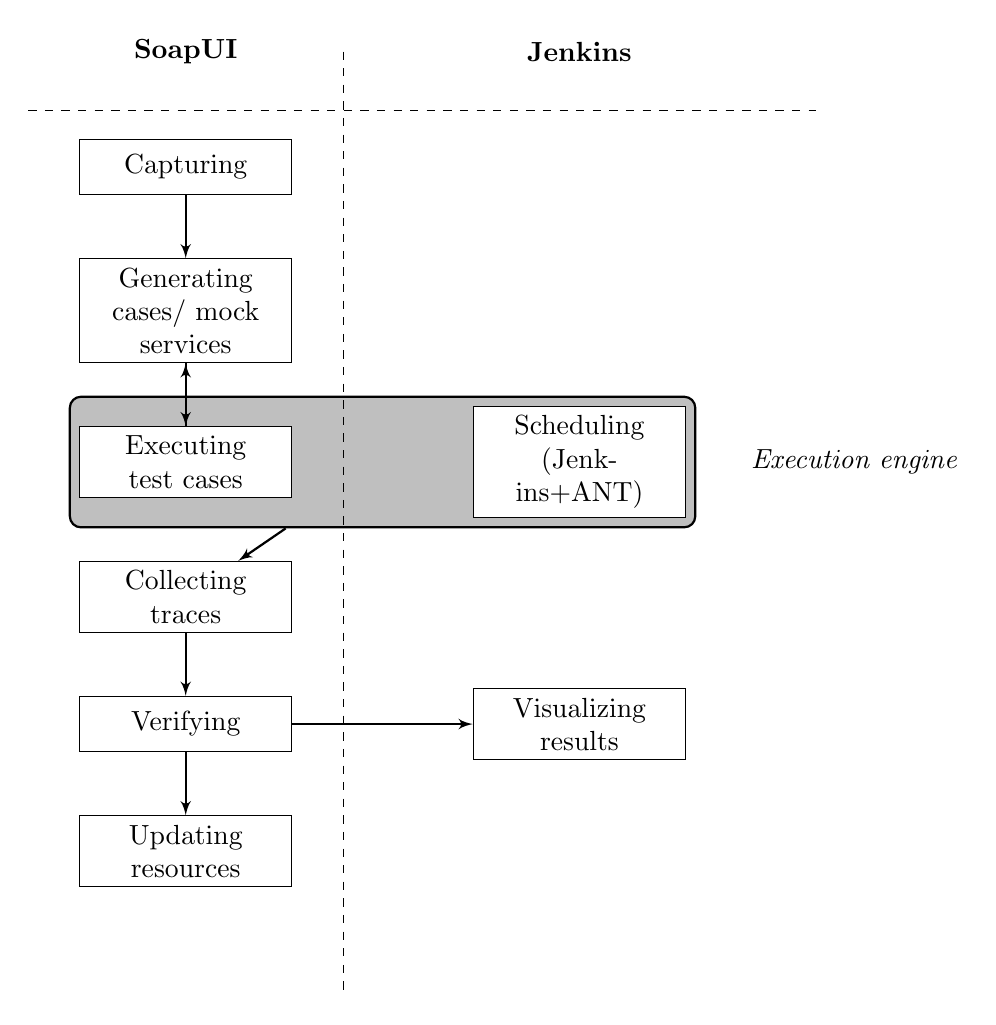
\begin{tikzpicture}[
    start chain=going below,    % General flow is top-to-bottom
    node distance=8mm and 50mm, % Global setup of box spacing
    ]
% ------------------------------------------------- 
\tikzset{
  base/.style={draw, on chain, on grid, align=center, minimum height=4ex},
  label/.style={on chain, on grid, align=center, minimum height=4ex},
  proc/.style={base, rectangle, minimum height=2em, text width=7em, fill=white},
  box/.style={draw, thick, minimum height=4em, fill=lightgray, rectangle, rounded corners},
  line/.style={draw, thick, -latex'}
}
% -------------------------------------------------
% Placing the nodes

\draw [dashed] (2,0) -- (2,-12);
\draw [dashed] (-2,-0.75) -- (8,-0.75);
\node[label] (l0) {\textbf{SoapUI}};

\node [proc] (p0) {Capturing};
\node [proc] (p1) {Generating cases/ mock services};
\node [proc] (p2) {Executing test cases};
\node [proc] (p3) {Collecting traces};
\node [proc] (p4) {Verifying};
\node [proc] (p5) {Updating resources};

\node[label, right=of l0] (l1) {\textbf{Jenkins}};
\node [proc, right=of p2] (p6) {Scheduling (Jenkins+ANT)};


\node [proc, right=of p4] (p7) {Visualizing results};

\begin{pgfonlayer}{background}
  \node[box] [fit = (p2) (p6)] (b0) {}; % Execution engine
\end{pgfonlayer}

%\begin{pgfonlayer}{background}
%  \node[box] [fit = (p1)] (b1) {};      % Surrogate engine
%\end{pgfonlayer}

\node[label, right=3.5cm of p6] {\emph{Execution engine}};
%\node[label, right=4cm of p1] {\emph{Surrogate engine}};

\path [line] (p0) -- (p1);
\path [line] (p2) -- (p1);
\path [line] (p1) -- (p2);
\path [line] (b0) -- (p3);
\path [line] (p3) -- (p4);
\path [line] (p4) -- (p5);
\path [line] (p4) -- (p7);

\end{tikzpicture}
\caption{Technical framework implementation} \label{fig:structure}
\end{figure}
\end{comment}

\begin{figure}[H]
\centering
\includegraphics[angle=90,width=12cm]{oldframeworkWithTech.png}
\caption{Technical framework implementation} 
\label{fig:structure}
\end{figure}

In the framework architecture, SoapUI provides an environment for test resources (e.g. test cases and scripts) development and storage. With Jenkins the test engineer can configure and execute test runs withouth the need --- or possibility --- to tamper with test resource code. Restricting access to code is also a security measure. Those who only wish to examine the health of the systems can do so through Jenkins's graphical UI. 

The experiment quickly showed the difficulty of dividing responsibility between software components. Implementing a feature like test execution requires cooperation between tools where one assumes part of the duties while the other fulfils the rest. Depending on the observers perspective either in true irony or an illustrative example implementing the integration testing framework already creates a number of system dependencies.

Execution engine duties are split between the actual running of the tests and scheduling test cycles. The execution engine running the tests, SoapUI, also collects execution traces. These are transformed into legible form (simple text) and can be examined in the Jenkins UI. Visualizing the test results is considered implicit in the verification process.

\subsection{SoapUI}

\textbf{SoapUI}\footnote{http://www.soapui.org} is an integrated development environment, and used in constructing test scripts, both manually and through \emph{capture and playback}. Capture can also be used to to create scripts to simulate the behaviour of systems thereby satisfying the requirement of having a surrogate engine. Effectively, SoapUI uses capture for both test case \emph{and surrogate component} generation. These mock service or surrogates components allow verification by providing an otherwise absent execution trail or returning courtesy messages of the test outcome, or what has happened across the integration black box.

After their creation test cases can be run in SoapUI and the tool affords a program script that can be run on the command line simply by specifying which SoapUI project and which test suite or cases should be run.

Because specification of sufficient accuracy for deriving test cases automatically were not available, test cases are based on capture. Test cases are written in a SoapUI-tailored template format but since their structural composition is largely that of an XML file, their fair reusability and low risk of vendor lock-in is justified. 

Execution traces are simply full text accounts of test results. These include information on the test case level or which case failed, which is why tests should only have one assertion if possible as this helps seeing what exactly is wrong the program and where the defect might be \citep{duvall2007continuous}.

\subsection{Jenkins}

\textbf{Jenkins}\footnote{http://jenkins-ci.org/} is a continuous testing and integration tool which manages test execution for software projects. Running on a server, Jenkins can be triggered to run on a regular basis (e.g. daily, weekly, every hour) or immediately as new code is committed into a repository linked to a Jenkins project. Since test cases, suites, collections of suites can be linked to independent projects, it is easy to organize tests, tailor and schedule runs, and generally execute tests only when it is needed\footnote{A Jenkins project may be rigged to run any number of test suites which in turn can contain any number test cases. Projects can therefore be configured to test an area or areas of functionality --- or perform all tests.}.

It should be noted that Jenkins is made with software development rather than regression testing in mind but on balance the regression test set-up is equally effective. At the bare minimum, Jenkins is given a test case execution script courtesy of SoapUI which it runs in the native operating system's environment and collects traces provided by the cases and script.

Jenkins is used in conjunction with ANT, which while not necessary, is an industry best practice and contains advantages cross-system configuration. ANT is essentially an XML-format configuration file which specifies which steps are to be taken when a new build, i.e. updated version, is created. The build can be appended with software engineering tasks, including running a test execution script. 

\subsection{Performance testing}

Performance testing in the framework is done with SoapUI’s sister tool \textbf{LoadUI}\footnotte{\url{http://www.loadui.org/}}. Performance tests based on SoapUI test cases can be configured with the tool’s graphical UI. Assertions, such as threshold limits for response time, can be added to the cases to establish pass/fail criteria. The execution of load tests and integration to Jenkins are analogous to SoapUI. As with SoapUI, the tool provides a program which can be run from the command line with the test run details and conguration settings as parameters.

% muokka database kohta, ei ole laukkaen mallissa
% lisää kuva project - suite - case suhteesta?

\chapter{Evaluation}
\label{chapter:evaluation}

Chapter \ref{chapter:evaluation} compares the proof of concept construct to external requirements and guidelines, and considers how the framework satisfies criteria presented earlier in the thesis as well as any new concerns and observations.

\section{Heuristic evaluation of the framework}

The framework is evaluated mainly by qualitative measures, but a quick heuristic analysis is also used to validate to new model. This section compares the proposed framework to the requirements laid out in Section \ref{section:requirements}, and the presented framework models and framework theory.

\begin{description}
  \item[R1 It shall be possible to run test cases.] \hfill \\
 SoapUI has the necessary functionality to run cases on command. There is also a program with which cases can be run outside the application.
  \item[R2 It shall be possible to schedule automatic test runs.] \hfill \\
  Jenkins projects can be configured to create new builds regularly. The builds in turn can be configured to execute scripts, such as the one afforded by SoapUI, before each build.
  \item[R3 It shall be possible to write and generate test cases.] \hfill \\
  SoapUI is essentially an development environment and supports the creation of test cases.
  \item[R4 It shall be possible to capture and replay messages.] \hfill \\
  SoapUI has monitoring functionality which acts as a proxy and records and lists intercepted messages. Request messages can be rerun, if necessary.
  \item[R5 It shall be possible to generate mock services or stubs.] \hfill \\
  Messages recorded in SoapUI can be turned into cases or mock services through a wizard.
  \item[R6 It shall be possible to validate test results automatically.] \hfill \\
  SoapUI test cases can be supplemented with assertions for automatic verification.
  \item[R7 HTTP/XML, JDBC, and (S)FTP protocols shall be supported.]  \hfill \\
  The necessary protocols can be through web services already implemented in the SUT.
  \item[R8 It shall be possible to generate test loads, and conduct load tests.] \hfill \\
   Load tests are possible based on SoapUI test cases and surrogates, using the LoadUI sister tool.
  \item[R9 It shall be possible to generate test loads and conduct stress tests.] \hfill \\
   Stress tests are possible based on SoapUI test cases and mock services, using the LoadUI sister tool.
  \item[R10 It shall be possible to monitor test results and performance metrics.] \hfill
   LoadUI offers a dashboard and statistics view into performance metrics.
\end{description}

Compared to the models by \citet{liu2009unified} and \citet{huang2008surrogate} in Chapter \ref{chapter:frameworktheory} the new model covers most of the same ground with the addition of the surrogate component generation process. \citeauthor{laukkanen2006data}'s \citeyearpar{laukkanen2006data} framework includes test asset management as a responsibility area to control test cases and attached data. The framework could be extended with a database to manage test resources.
% Platform independennce not requirement for Wärtsilä, involved coding plugins and adapters, which should be avoiuded

\citet{fewster1999software} present key characteristics of an automated test regime, a system of government of testing which can be likened to a framework but with more emphasis on governance and rules of practice. Characteristics of a good test regime are:
\begin{itemize}
\item easy to select tests to be run at the touch of a button
\item tests take care of all their housekeeping such as environmental set-up and clear-down
\item it is easier to add a new test to the automated pack than to run that test manually
\end{itemize}

The framework satisfies the first criteria easily. Executing packages of tests packages in Jenkins is done with a simple click. Likewise choosing which tests to execute is not uncomplicated. Integration test cases can be organised inside Jenkins projects so that only the needed cases are run. This does call for some maintenance work, however. It is essential to know which projects should be appended with the new case. Otherwise the unorganized collection of test cases becomes clumsy to use. This issue can be subverted by guidelines already at the test creation process so that the test engineer adds the case in the correct test suite. The framework administrator meanwhile sees to that each suite is correctly linked to projects.

Automated testing already requires the second criteria be satisfied. Assuming the test server and SUT servers are available, and test cases contain necessary information to access information services, the test set-up is complete. Because some features require inputting information, like creating test orders, which cannot be allowed in production, mock services are used. Here, test messages travel through the same \emph{"integration black box"} as actual messages would, and the only part that is not "real" is the end point system the testing of which is outside of integration test scope. Therefore the described test approach provides an accurate result of integration functionality and health. Not part of the automation, a test engineer should monitor execution and react appropriately in case a test case fails.

As for the third criterion, running a test manually and adding the test to the automated pack both require writing or generating the case first. With a good template and guidelines in place, the case writing task can be expedited and the engineer adds the case to the correct suite where it will automatically be picked up by the test scripts run through the framework.

\section{Qualitative evaluation --- Workshop}

% should there be more requirements in the background section, add interviews summarize succinctly

% should there be interviews about what is wrong with testing now
% ville: health check
% paavo: 
% eero: protocols, requirements
% why interviewees slected

Qualitative evaluation of the new framework was performed through interviews with Wärtsilä's experts in a workshop, supplemented by observations of the framework prototype. 

The workshop was organized to showcase the new framework model to experts and interested parties inside Wärtsilä, and to evaluate its applicability in the company. The purpose of the event was twofold: to \emph{validate} and \emph{improve} the framework hypothesis. Feedback both critical and supportive was elicited and suggestions for further improvement collected. The workshop event was facilitated by the author.

A total of seven poeple attended the workshop: two technical experts, a testing expert, and three members of a partner's infrastructure team and the author. The partner members and one of the technical experts joined the meeting via remote access. The meeting agenda and purpose was explained to all participants beforehand, and the discussions recorded with the workshoppers' consent so that they could be comprehensively analysed afterwards.

The most sought-after results of the workshop were the observations of people who are actually to use the framework should it be adopted, and how they view creating test cases, managing test results, or otherwise maintaining the framework.

\subsection{Testing validation}

At the beginning of the meeting, participants were presented with a mission statement and a short introduction to the topic explaining the reasons that led to commissioning an automated testing framework study. The subject of current testing was brought under discussion by the technical experts. 

The first technical expert said that for her, testing mostly consists of code inspection, a white-box testing method not investigated or included in the framework. Code inspection is done by the developer to find issues in the code directly, without actually executing it. The expert also added that the lacking \emph{negative testing}, or testing cases that are expected to fail to see if ill-formed input is able to disrupt systems, was a problem. 

The remaining parties quietly agreed with the current testing status that was presented which stated that testing is largely ad hoc and driven by each project in its own way. The testing expert and technical expert jokingly referred to testing being a mandatory step whose purpose is not so much to uncover bugs but to prove systems are ready for the next go-ahead. While the veracity of such a claim is dubious, a framework can serve to ensure proper testing by communicating that negative cases should also be added to testing scope.

\subsection{Requirements validation}
\label{subsection:requirementsvalidation}

Following the introduction to Wärtsilä testing, the collected framework requirements (see Section \ref{section:requirements}) were shared with the intent to validate them again, and determine the most important ones. The first technical expert put most weight on the requirement demanding test generation (R3) or automatic creation. Concern centred on the labour cost of creating tests and generation was crucial in making larger scale testing economically feasible. While the generation requirement may be argued to be not the most important component of a testing framework per se, it clearly sparked excitement among the participants. The requirement has a lot of potential for gains.

The testing expert was more concerned if the framework actually provided any actionable results. Therefore, the requirement for automatic test results validation (R6) was named the most important. If the framework could not contribute to fixing defects in the integrations and making systems better, it would have little value. Automating this step was also important because otherwise the crucial decision of whether the test passed or failed would have to be done manually. The discussion continued on the theme of reporting failures. The testing and first technical expert toyed with the idea of creating automated bug reports in the framework and forwarding them to the bug tracker. This was added as a new requirement (R12) for the framework.

The second technical expert agreed with the previous comments citing both requirement 3 and requirement 6 as the most important. Meanwhile, the partner members underlined the importance of performance tests (requirements R8 and R9).

Throughout the discussion the addition of new requirements was welcomed. Along with automated bug reports, one clear new requirement was version control. Systems and environments go through changes and test results always pertain to one particular version. This information must be easily available and understandable. Moreover, it is useful to document in which version of the system and environments the captured test cases or surrogates were generated. Version control was added as requirement eleven (R11).

\subsection{Framework use and maintenance validation}

The issue of framework maintenance was raised by the testing expert. Because the proposed framework required test generation using capture, test resources would have to be updated after any change in the systems' behaviour that would render them moot or possibly even misleading. This was also a principal concern in the criticism of capture and replay discussed in Chapter \ref{chapter:frameworkanalysis}. After discussing the matter with the technical experts the workshop participants concluded that test reusability would be high because test cases would only have to change very infrequently. Hence, capture was accepted as a cost-effective way to create test resources. The biggest automation pitfall was bypassed.

The framework model (see Figure \ref{fig:structure}) was broadly accepted. One partner expert pointed out that the model explicitly prescribed a database for test resources where any filing system would have sufficed. The participants agreed to remove this technical prescript. The connecting arrow between "updating" and the test resource library was also ambiguous in that it did not distinguish between adding a new test case or mock service the library or updating test results and logs after a testing event.

The demo was also met with appreciation. While agreeing in principle, the participants were eager to pilot the prototype to see how it fit into the company's way of working. The framework terminology should also be replaced with terminology used at Wärtsilä.

An alternative suggestion for the implementation also surfaced in which testing would be done through the existing message monitoring tool. The monitoring tool already makes records of messages before and after integration transformation and had the functionality of resending recorded messages. This promising alternative is explored more in Chapter \ref{chapter:discussion}.

\subsection{Summary}

The framework was an encouraging step forward in the adoption of the automated integration testing framework. The workshop yielded two new requirements while highlighting some the testing concerns outside the scope of the framework. The stakeholders now informed, piloting the framework can continue.

Wärtsilä should continue to work towards affirming which solution or product best satisfies its needs. The monitor tool -based solution suggested during the workshop is a viable option. The monitoring tool can already record and replay, but a test case generation harness, UI, and performance testing solution remain unsatisfied. Commercial tools can also be evaluated through trial licenses with reasonable expense.

The most important findings of the evaluation were:
\begin{enumerate}

\item High level of test resource reusability supports capture and replay
\item New REQ11: Version control in naming test resources (cases, environments, mock services)
\item New REQ12: Integration to bug tracker (email report)
\item Negative testing should be included in testing scope
\item Framework should be piloted in a project
\item Align framework to Wärtsilä way of working
\item Harmonize framework terminology
\item Code inspection as a way of testing
\item Having a test "library" rather than "database"
\item Use resources already available: monitoring tool based test framework
\item "Update resources" process box has ambiguous links in the framework figure
%\item Test coverage who supports who tests, 
%\item Curiosity over test tool selection
\end{enumerate}
%%%%%%%%%%%%%%%%%%%%%%%%%%%%%%%%%%%%%%%%%%

The participants agreed to a follow-up meeting where topics like adopting and piloting framework and the monitoring tool alternative could be further discussed. 

Based on participant feedback the framework was updated and is shown in Figure \ref{fig:newframework}. 

\begin{figure}[H]
\centering
\includegraphics[angle=90,width=9cm]{newframework.png}
\caption{Updated testing framework hypothesis}
\label{fig:newframework}
\end{figure}

The updated test framework contains an additional step for the new requirement of sending automated bug reports. The test database is now called a library since resources are not simply static values. These, along with the rest of the new improvement ideas, remain to be implemented.

% All the discussion was taped and the participants were given Post-it notes to write down all ideas that surfaced during the workshop. In total six persons - consisting of developers from maintenance, team leaders and one senior manager - attended the workshop.
% Goals - applicability of the model, questioning it
% validate and improve

% teknisempi kuvaus? kenellä on nyt integraatiovastuu ja kuka testaa 
% research method

\chapter{Discussion}
\label{chapter:discussion}

Discussion is divided into three parts. In the first the framework construct is deliberated and discussed. In the second, interesting topics and concerns are brought under light and analyzed. The third part critiques and addresses the limitations of the study.

\begin{comment}
- the mixing of manual and technical aspects
- examples of technical, contextual needs, flexible software
- manual, involving stakeholders and getting support, maintaining the model
- the result is generalizable in parts at least (manual process part that is)

- integration testing neglected subject
- staging post or more
- component testing
- doing away with integration, testing as software grows
- responsibilities per integration, difficult to maintain otherwise, whose responsibiltiy?
- getting to the beef - a compromise

- capture replay remains debateable
\end{comment}

\section{The framework construct --- man or machine?}

%mixing manual and technical aspects
One of the fundamental difficulties in developing an automated integration testing framework is making sense the technology and manual process relationship. The two are hopelessly intertwined. Clearly as a framework for \emph{automated} testing the framework is realized by algorithms and brute computing power, but such a tool cannot be wielded successfully without human intervention and maintenance. It is this blurred relationship of man and machine, the delicate mix of technological configuration and human work process model, which tries the framework designer and which also motivated the researcher.

Harking back to the \citet{pezze2008software} definition of a \emph{"circuit board with empty slots for components"} is useful here. The framework consists of roles or slots to be filled by applications or manual processes, the choice being left to each individual testing project. The framework will fail if it is too narrow and incompatible or too broad and poorly supported.

The Wärtsilä framework allows extension and accepts new test cases or surrogate components for a predefined set of protocols. The circuit board is then fleshed out for each project individually. Tests can be divided into groups so that only the ones that need to be executed can be invoked. Test packages can each be configured to run at their own intervals. The framework adapts to testing need while retaining the same testing process and technical form.

% manual challenges and adaptin the framework
Confirmed in the empirical part the thesis, an essential challenge is fitting the framework into the target company's way of working. Testing organization requires the cooperation of many individual stakeholders. In Wärtsilä's case this contribution was seen as extra work for solution managers and soliciting their support was difficult. It is natural that the final development and adoption of the integration testing framework happens in strict co-operation with the key stakeholders.

The great bulk of the manual work belongs to the preparatory step of the framework and is required at the early stages of testing. Here, a clearly defined framework which states what resources or contributions are needed can bring credibility and trust to the project and provide a channel for cooperation. The kicker to having this kind of documented process and automated framework is the reusability of test resources like test cases (also a prerequisite of automation), which may act as an incentive to contribute to the framework for the stakeholders. This remains to be seen, however. Admittedly, cases will have to be maintained and updated.

It is worth noting that the thesis does not make any explicit recommendations as to which aspects of automated testing should be measured and used as key indicators. The metrics are context-specific and may include anything from number of test cases, passed tests, failures, bytes taken, coverage, etc. Fortunately, many of these can be collected and quantified easily.

% component testing replacing integration testing

\section{Topics for further research}

Software is abstracted and managed by splitting it to blocks or components. These blocks form a specific functional area that is a thematic whole and which can be assigned to responsible and which generally make the software easier to manage. In fact, integration might be thought to be not between systems but between software components, which respects interfaces more broadly. One may ask if integration testing scope will become too bloated in this vein of thought any transaction with two points constituting an "integration".

% getting rid of the word integration literature
It is possible that \emph{integration} is a misleading term. Sometimes testing is divided to unit, component, and system tests as opposed to the traditional unit, integration, system paradigm \citep{myers1976software, pezze2008software}. Supposedly, a component is a combination of simple units and system tests focus on testing when all necessary components have been integrated. Testing grows with development as the size of the software blocks grow (call the units or components or whatever). But the target of testing is entirely removed from the semantics of this division. Which type of functionalities should be tested and where should the testing focus be?

% where's the beef? testing often and testing early. component based. integrations should have responsible people.
% tired old big-bang as an alternative
% future: fault-based testing
In practice, "integration testing" might be skipped entirely in favour of end-to-end system tests which are thought to cover testing integrations. Once again testing is squeezed. Consequently, another area begging attention is whether integration testing should be conducted through end-to-end testing and what are the potential upsides and downsides. More accurately, this is to ask if integration testing should simply concentrate on the integration between two systems, or if a whole chain of trans-system communication should be packaged into a test case. The trade-off is between having simple or representative cases: an end-to-end test case will give more coverage per case, and perhaps a more realistic test scenario, but also include a larger testing scope. If something goes awry, can the test engineer or developer easily see what's wrong? \citet{duvall2007continuous} advocates including only one assertion per case, which is counterproductive relative to the scale of an end-to-end case. If only a portion of system communication is relevant, the rest goes to waste.

% capture playback and model generalizability, future resarch
% citations?
A key enabler of automation, \emph{capture and playback} is a frequent target of criticism but many commercial and non-commercial testing tools are based on it. Theoretically it may not be the best option, it arguably satisfies most companies' testing requirements and needs, at least temporarily. It remains to be seen if public opinion shifts after more is known about the lifecycle of such a tool and the maintenance requirements of such a strategy. The alternative, model-driven testing, requires an initial investment that is greater, but it might pay off. Perhaps system modelling will become so easy, and the philosophy of separating content with structure so prevalent as to enable test case and test data creation based on specifications.

Future research might also labour over collecting, combining, and comparing strategies for test case creation. As such, experiments and proof of concepts have been given for generating test data \citep{linnenkugel1990test}, creating test case templates automatically \citep{bai2005WSDL}, and capture strategies \citep{meszaros2003agile}. This work should be catalogued and analyzed.

\citet{rehman2007testing} have done commendable work stepping back to examine integration testing through fresh eyes. Different practical alternatives for testing \emph{component integrations} are laid out and compared in the 2007 article. A similar unbiased and novel approach should be applied to reappraising the tired old big-bang and integration strategy in general taking stock of the alternatives that exist.

More focused areas like fault-based testing also merit research. The framework might be supplemented by a set of guidelines for creating fault-based test cases, for instance. This means creating tests cases based on defects detected in the system.

Finally, it is not possible to go through every code branch or to test every possible input sequence. As \citet{myers1976software} put it, testing is a problem in economics. Test cases must provide a maximum yield on investment, where yield is measured as the probability that the case uncovers a new defect. \citep{myers1976software} Implementing a testing framework is essentially a software development project with all associated risks and costs \citep{kaner1997pitfalls}. 

% rehman focusing on components but includes unit-integration-system

\begin{comment}
Future research:
capture playback popular still despite warnings, what's up? when is it not applicable?
relationship between automation and manual work, test automation manual maintenance
integration test strategy in the vein if rehmann, what options/technical strategies are there? tired old big-bang
Strategies for test case creation (zeng & tan 2013)
study merits of fault based testing for more efficient tests
distinction between a technological configuration and process model is difficult.

notion of unit to system antiquated, block to block also
more an issue of test case construction and traceability
end-to-end tests are adequate if they can point to problem code accurately
\end{comment}

% future building software automatically producing models and specs for automation and generation

\section{Limitations}

Well begun may be half done but the integration testing framework is not fully fledged and ready to be adopted for immediate use. At the very least it must be piloted in a project and streamlined to fit Wärtsilä's ways of working and any technical glitches ironed out. Although it met its requirements, the framework itself was not subjected to large scale testing. 

Perhaps more importantly, the benefits and costs related to other technical solutions, such as the one based on the monitoring solution, need to figured out, too. The testing framework process is generic and can be implemented by different practical solutions. The construct was based on free and open source technologies but shifts in the tool landscape or taking into account the whole lifecycle of the tool technologies may incur unexpected costs.

The framework was evaluated by mostly in-house experts whereas the actual testing effort may in fact be conducted by Wärtsilä's external suppliers and partners. Imposing practices to these stakeholders without consultation is surely unwise and subsequent framework implementation should be carried in co-operation with key stakeholders.

It is also worth noting that the thesis does not make any explicit recommendations as to which aspects of automated testing should be measured and used as key indicators. The metrics are context-specific and may include anything from number of test cases, passed tests, failures, bytes taken, coverage, etc. Fortunately, many of these can be collected and quantified easily by the framework components.

Lastly, it should be noted that the thesis's recommendations and construct are applicable to Wärtsilä's case only, though the research offers more general guidelines and observations as well.

\chapter{Conclusions}
\label{chapter:conclusions}

This thesis has grasped disparate threads from academic literature and woven them into a solid piece of fabric tested in real organizational settings. The thesis asserts that the devised framework presented in Chapter \ref{chapter:frameworkproposal} is generalizable and can benefit any party doing testing based on capture and replay. Testing as a process, is cemented in three steps, preparing necessary input and conditions, executing tests, and verifying results, perhaps with the addition of a clean-up step logging test results or creating test reports. The study results are based on comprehensive analysis and evaluation through multiple criteria.

The hallmarks of constructive research were also met successfully. The thesis brought a real problem under theoretical scrutiny and generalized it into a model which was subjected to testing. The results of the empirical study were evaluated and discussed and returned to academic context.

The framework construct satisfied the case company requirements while respecting testing practices and theory. The practical functioning of the framework was presented through a proof of concept prototype evaluated by company experts and compared to previous prototypes. While the framework is generalizable the implementation is context-specific, which must be kept in mind when conducting further evaluation of the automated testing framework at the target company. Previous research proved intelligent integration testing frameworks are possible, but the thesis makes this \emph{plausible}.

Looking at the research questions again: \\

\begin{adjustwidth}{2.5em}{0pt}
\textbf{1. What are the requirements for an automated integration testing framework?} \\
\end{adjustwidth}

Testing framework requirements include a test case generator, a test harness (that is to say necessary surrogate components and possibly a surrogate generator), a test engine, and an oracle verifying test results. The generation can be based on capture replay or formal models both of which allow for automation. While test execution is automatic, the creation will likely remain a mostly manual task. To create and manage the cases or surrogate components, the framework essentially calls for an environment in which to develop these test resources. The environment is typically capable of executing tests as well. The test oracle incorporates service logic that examines test outputs and execution traces to determine success or failure. Often logic statements about success or failure, assertions, are embedded directly into the test cases with possible external resources such as expected results stored in a database. 

Requirements specific to Wärtsilä are listed in Section \ref{section:requirements} and further evaluated in Section \ref{subsection:requirementsvalidation}. \\

\begin{adjustwidth}{2.5em}{0pt}
\textbf{2. How should the testing framework be constructed and maintained?} \\
\end{adjustwidth}

The second research question is answered in part by the framework construct. The framework structure is dependent on the three core processes: generation, execution, verification, as well as the available or suitable tools. Special attention must be paid in adopting and aligning the framework inside the target organization.

Maintenance consists of the creation of new tests for new or changed integrations. As the rate of change in Wärtsilä integrations was deemed infrequent, the rationale for automation was high. The creation of test cases is the most labour-intensive maintenance task and Wärtsilä should support this both to increase the efficiency of the maintenance work and to make sure the framework is correctly configured. The guide documentation should also explain the test package structure and how the test cases should be stored so that the framework can find them.

Text execution occurs through a graphical UI, or, or more often, automatically. The automation half of the framework (see \ref{fig:newframework}) is exempt from maintenance. Naturally, the use and configuration of the tool should be included in the framework guide.

One of the essential findings of this thesis is that Continuous Integration bridges the gaps in integration testing theory when examining the entire software lifecycle. Authors like Myers and Fewster and Graham \citep{myers1976software, fewster1999software} as well as textbooks \citep{burnstein2003practical} still continue to perpetuate the image that integration testing is mere a software component assembly task and simply a staging post in software development. This is unfair because integrations should be tested regularly when there is even the slightest change in systems composition or source code. CI connects integration testing with functional, non-functional, and regression testing while adhering to the tester's adage "test early and test often". CI also requires automation to enable the continuity of testing.

Good testing is based on good plans, such as specifications of systems and models of their behaviour, and ensured by good governance. Though a virtue in the own right, technology has even made it possible for formatted plans to be translated into program logic directly, echoing the separation of structure and content. The structure is a generalizable asset replicated in tests and content is the test data. A good example of this is web services where a single specification file can be used to generate an executable test case. However, test data and verification (adding assertions and the like) must be done by a test engineer, still. It remains a task for human discretion to decide what is to be tested and what the testing objectives are.

% Good planning is required and ensured by good governance and realized by a well-documented process model and carried out in practice by a technological framework. The strategy-operation alignment process goes through many gates and finding the right fit is not easy.

\begin{comment}
% pezze integration faults
Inconsistent interpretation of parameters or values
Violations of value domains or of capacity or size limits
Side-effects on parameters or resrouces
Missing or misunderstood functionality
Nonfinctional problems
Dynamic mismatches
\end{comment}

\begin{comment}
Interpretation
    wrong function - something else than specified
    extra function - more than what is expected/needed
    missing function - not all that is specified
Miscoded call (error which causes the developer to place the call instruction at the wrong point in the program)
    Extra instruction fault: the call instruction is on a path which should not have the call.
    Wrong placement fault: the call is at the wrong location on the path which should have the call instruction.
    Missing instruction fault: the call instruction is missing on the path which should have the call.
Interface error
    When stardards or agreements are violated
\end{comment}

% ERRORS: wrong function, extra function, missing function 
% Miscoded call error
% Interface error (Lueng \& white) 
% =================================================

% Thin threads, groupin into a tree (tsai et al)
% Test data difficult to select (linnenkugel mullburg)
% add background informtion: general about regression/integration/software testing, ITIL processes at Wärtsilä
% and possibly more...

% Load the bibliographic references 
% ------------------------------------------------------------------
% You can use several .bib files:
% \bibliography{thesis_sources,ietf_sources} 
\bibliography{ref} 

% Appendices go here
% ------------------------------------------------------------------
% If you do not have appendices, comment out the following lines
\appendix
% \input{appendices.tex}

\begin{comment}
\chapter{Workshop invitation and agenda}
\label{chapter:first-appendix}

\scriptsize
\begin{tt}
You are cordially invited to: \\
\\
Integration Testing Workshop 
12.6.2013, 10 am (EET time) at Wärtsilä main office, Helsinki and Live (I will let you know about the room shortly) \\
\\
In the workshop we will review a new prototype framework for automated regression testing of Wärtsilä's system integrations. As a major stakeholder, your participation is important and would be much appreciated. \\
\\
***Meeting agenda*** \\

Presentation: Model for continuous integration testing \\             

Model evaluation and discussion: validate \& improve \\

Coffee break \\

Demo: Technology proof of concept: SoapUI+Jenkins \\

PoC evaluation and discussion: validate \& improve \\
\\
The workshop will take about two hours all in all.\\
\\
I hope to secure your participation because it is important all stakeholder groups are represented in the event and have the opportunity to further develop the framework and work processes. This will yield the best result and pave the way for future success. \\
\\
Thank you for your consideration. If you have any questions please do not hesitate to contact me. \\
\\
Looking forward to seeing you,\\
Antti Heikkonen\\
Thesis Worker\\
Wärtsilä Corporation\\
Helsinki
\end{tt}

\end{comment}

\normalsize

\chapter{Guidelines document}
\label{chapter:guidelines-appendix}

\emph{NB: Sensitive information in the guideline document has been blotted out.}

\section{Introduction}

The following document gives guidelines and recommendations in testing Wärtsilä’s system integrations. It is based on the author’s master’s thesis research and experiments at the company during the Spring of 2013. 

The distilled wisdom to come is not argued in lengthy detail and anyone interested in additional information or analysis is invited to read the thesis which is available at: \url{<http://dippaeditor.com/preview/eVW29cQ7gwyM/>}

In this guideline document the reader is first presented with the key finding of the research – a process for integration testing on which the technical testing framework is implemented. Next, guidelines on general integration testing strategy, test resource management and preparation, test execution, and result verification are given. The compiled guidelines are grounded in a lifecycle perspective and take into account maintenance issues. Based on the thesis prototype framework, illustrated step-by-step instructions for test case construction are also provided.

\section{Recommended test process}
The test process is divided in to a preparation step where test resources are created and an execution step in which test cases are run and rerun as the step is repeated. The whole process is pictured in Figure \ref{fig:app_framework}.

\begin{figure}[H]
  \begin{center}
    \includegraphics[width=13cm]{framework.png}
    \caption{Test framework}
    \label{fig:app_framework}
  \end{center}
\end{figure}

Testing begins with capture in which records of message transactions that are used to create a test case or mock service so the message exchange can be re-executed in the test environment.  New cases are proofed to see if they work and then committed to the test library.

Cases are packaged into suites and suites divided into test sets which are configured to be executed automatically at regular intervals. Test logs and failed outcomes are also stored in the test library. If a bug is found an automatic report is sent to the bug tracker.

The recommended test process is described in more detail in the thesis Chapter \ref{chapter:frameworkproposal} and \ref{chapter:evaluation}.

\section{Recommendations}
The following chapter gives recommendations for integration testing practices based on the research conducted at Wärtsilä. Recommendations are divided to general advice, recommendations in managing test cases, considerations in test case execution, and finally comparison/ verification precepts.

\subsection{General strategy}

\begin{description}
\item[Plan coverage and relevant measures beforehand.] \hfill 
\\
Define the test scope and roles, and solicit support from the parties that need to be involved in creating e.g. test cases. Relevant measures should be identified to set the stage and guide the whole implementation of the test framework.
\item[Use capture/replay.] \hfill 
\\
Broadly speaking there are two general ways to satisfy the requirement of test case generation: capture/replay and model-based testing. The former is the better option in testing Wärtsilä’s system integrations because of cost-effectiveness: Based on experts’ statements integrations do not undergo many changes and therefore costly test resource maintenance work is minimal. Conversely, building sophisticated, machine- interpretable formal models for automatic test case extrapolation requires more investment upfront and is risky.
\item[Draw call graph to visualize integrations.] \hfill 
\\
A call graph is a tool to visualize integrations. It should include systems, integrations, and different transactions passing through the integrations as well as any additional technical information. Note that the purpose of the call graph is not to document the technological specifics of integrations, but to discern dependencies and plan test scope.
\item[Use continuous integration tool for automated test execution.] \hfill 
\\
Longer term goal to adopt continuous testing in development as well. Continuous integration provides the best quality in testing because bugs are found  and addressed as soon as they manifest themselves in the systems. Continuous integration also makes the most out of automated execution through frequent, systematic, and comprehensive test runs. In the future, continuous integration and test resources can be used already at the development stage benefitting the construction of new systems or the improvement of old ones.
\end{description}

\subsection{Test case management guidelines}
\begin{enumerate}
\item Keep number of cases low. More cases means more maintenance work.
\item But keep granularity high. Cases can be handpicked and queued to test just the right things. 
\item Prune cases periodically. Make sure they are up-to-date. Eliminate unnecessary ones that cause extra work.
\item Check that there is no overlap. Redundant cases create problems in for example traceability (which case was run) and maintenance (which case was updated).
\item Limit the number of assertions or comparisons per case. If the case fails, it is quick and easy to find the cause of the failure.
\item Organize cases into logical sets and execution suites. This helps find the right cases and organize execution. Tests should be organized around features whereas suites should be based on test goals. Make sure test resources are added to the correct sets or suites.
\item Make test resources easy to find. Use a centralized repository and make sure cases and other resources are commented and have enough meta-information to support searches.
\item Choose a data format that is simple (low memory requirement) but practical (e.g. can be used by tools, are based on universal standards).
\item Store test results thriftily. Keep log information on what has been tested, but only keep test results from failed test runs.
\item Think of ways test scripts can be optimized (e.g. check and stop execution if test environment unavailable).
\end{enumerate}

\subsection{Test case execution guidelines}
\begin{enumerate}
\item Assign test execution responsibilities: who is responsible for that certain features are tested.
\item Provide instructions how to use SoapUI for the creation of test resources or Jenkins to execute tests. (See end of this guide for step-by-step examples.)
\end{enumerate}

\subsection{Test result comparison/verification guidelines}
\begin{enumerate}
\item Remember that matching outcomes to previous outcomes is tricky. Dates and timestamps change.
\item Document comparisons so whoever uses them understands what they do.
\item Agree on and adhere to sensible naming conventions.
\item Keep comparisons simple to make updates and changes easier to do. 
\item For complicated or lengthy comparisons think if they can be simplified, or if manual comparison would make more sense.
\item Standardize to create reusable building blocks for constructing the comparison logic statements (e.g. reusable filters and regular expressions).
\item Use a balanced mix of sensitive and robust comparisons. If required by testing objectives, create different test cases for the two so they can be run separately.
\item Divide and conquer: create separate comparisons for each feature for easy set-up and matching to testing need.
\end{enumerate}

\subsection{What to test first?}
Implementation priority could for example be based on the following criteria:

\begin{description}
\item[Tests that are explicitly deemed important.] \hfill \\
E.g. some area that critical, has been recently changed, is prone to bugs or is known to have caused failures.

\item[A set of breadth tests that roughly cover all features in test scope.] \hfill \\ 
This will give minimum satisfaction of test objectives.

\item[Test for most important functions.] \hfill \\
Function importance may be attributed to e.g. message traffic, financial impact, etc.

\item[Tests that are easy to automate.] \hfill \\
Good for quick wins and return for investment. Also quickly ramps up the framework construction.

\item[Test that will give quickest payback.] \hfill \\ 
Implement test cases in projects which would otherwise require a lot of manual testing.

\item[Test that are run most often.] \hfill \\
If tests need to be run often, the tested area is likely subject to many changes thereby increasing risk.

\end{description}

\section{Example 1 –-- Configuring SoapUI with web service}
See Figure \ref{fig:app_configuringmessage}.
\begin{enumerate}
\item If you already haven’t, install the free version (not the pro version) of SoapUI from \url{<http://www.soapui.org/>}.
\item For a SoapUI sample integration create a new project in SoapUI. Right click the project and choose “add WSDL” and add the web service description (e.g. the one attached to this document).  This creates a web service binding with a sample request. 
\item The request is missing test data which must be added. For the attached example service for instance, insert the following in the fields with ‘?’ in this order: \censor{‘3333’}, \censor{‘32’}, \censor{‘GEN’}, \censor{‘False’}, \censor{‘True’}.
\item You must also add username \censor{ext_sco} and password \censor{wm7qa} in the ‘Aut’ authentication tab.  The test client must have the rights to access SUT services.
\item Add the correct endpoint URL in the request edit window, e.g. for the example service: \\ \censor{wesbqa.wartsila.com:5557/ws/sco.common.ws:SCOServiceProvider}.
\item Now the request can be run by clicking the green arrow. You should get a return message with engine information.  
\end{enumerate}

\begin{figure}[H]
  \begin{center}
    \includegraphics[width=13cm]{configuringmessage.png}
    \caption{Configuring the message}
    \label{fig:app_configuringmessage}
  \end{center}
\end{figure}

\section{Example 2 --– Creating and running a test case}
See Figures  \ref{fig:app_monitoringtraffic},  \ref{fig:app_addingassertions}, and  \ref{fig:app_testrunnerexecution}.
\begin{enumerate}
\item Right click the project you created and choose “launch SOAP monitor”. Use the default port and check the checkbox “use as global proxy”. 
\item Then open the sample request with test data and run it. This should create a log entry in the monitor window. 
\item In the monitor window click the button “add selected requests to test case”. Create new suite and test case in the wizard. Don’t leave any spaces in their names however!
\item Now, if you open the test case and test step you can find “monitor request 1”. Add an assertion or two (click ‘Assertions’ to open the assertion view), like SOAP message or SLA level. Run the case again to see that it passes.
\item Try running the case by right clicking the project and choosing ‘launch testrunner’. Run the new suite and case. The subsequently opened dialog provides the command with parameters to run the case from command line (it is at the top, scroll there).
\end{enumerate}

\begin{figure}[H]
  \begin{center}
    \includegraphics[width=13cm]{monitoringtraffic.png}
    \caption{Monitoring traffic}
    \label{fig:app_monitoringtraffic}
  \end{center}
\end{figure}

\begin{figure}[H]
  \begin{center}
    \includegraphics[width=13cm]{addingassertions.png}
    \caption{Adding assertions}
    \label{fig:app_addingassertions}
  \end{center}
\end{figure}

\begin{figure}[H]
  \begin{center}
    \includegraphics[width=13cm]{testrunnerexecution.png}
    \caption{Testrunner execution}
    \label{fig:app_testrunnerexecution}
  \end{center}
\end{figure}

\section{Example 3 – Configuring Jenkins} 
See Figure \ref{fig:app_jenkinsconfiguration} and \ref{fig:app_jenkinsprojectview}.
\begin{enumerate} 
\item Installing Jenkins is easy. Just download the war-package and deploy it on the test machine. Follow the instructions at \url{<http://jenkins-ci.org/>}. Afterwards open Jenkins at localhost:8080.
\item In Jenkins, choose new job, give it a name, choose freestyle project and OK. 
\item Next, configure the Jenkins project to run windows bat file at every build. Paste the command given by SoapUI testrunner and before it add a line were you change directory to the folder where SoapUI’s testrunner.bat is located. For the setup to work SoapUI must be installed on the same machine as Jenkins.
\item Building the project is now possible. If you keep Jenkins running, you can schedule builds, too, in the project configuration window.
\end{enumerate}

\begin{figure}[H]
  \begin{center}
    \includegraphics[width=13cm]{jenkinsconfiguration.png}
    \caption{Jenkins project configuration}
    \label{fig:app_jenkinsconfiguration}
  \end{center}
\end{figure}

\begin{figure}[H]
  \begin{center}
    \includegraphics[width=13cm]{jenkinsprojectview.png}
    \caption{Jenkins project view}
    \label{fig:app_jenkinsprojectview}
  \end{center}
\end{figure}

\section{Performance testing}

Performance testing can be done with SoapUI’s sister tool LoadUI (see \url{http://www.loadui.org/}). Performance test based on SoapUI test cases can be configured with the tool’s graphical UI. Assertions, such as threshold limits for response time, can be added to the cases to establish pass/fail criteria. The execution of load tests and integration to Jenkins are analogous to SoapUI. As with SoapUI, the tool provides a program which can be run from the command line with the test run details as parameters.


% End of document!
% ------------------------------------------------------------------
% The LastPage package automatically places a label on the last page.
% That works better than placing a label here manually, because the
% label might not go to the actual last page, if LaTeX needs to place
% floats (that is, figures, tables, and such) to the end of the
% document.
\end{document}